\documentclass[fleqn,usenatbib]{mnras}
\usepackage{newtxtext,newtxmath}
\usepackage[T1]{fontenc}
\DeclareRobustCommand{\VAN}[3]{#2}
\let\VANthebibliography\thebibliography
\def\thebibliography{\DeclareRobustCommand{\VAN}[3]{##3}\VANthebibliography}
\usepackage{graphicx}
\usepackage{amsmath}	
\let\Bbbk\relax
\usepackage{amssymb}	

\newcommand{\ha}{\hbox{H$\alpha$}}
\newcommand{\hb}{\hbox{H$\beta$}}
\newcommand{\oii}{\hbox{[O\,{\sc ii}]}}
\newcommand{\oiii}{\hbox{[O\,{\sc iii}]}}
\newcommand{\nii}{\hbox{[N\,{\sc ii}]}}
\newcommand{\sii}{\hbox{[S\,{\sc ii}]}}
\newcommand{\hii}{\hbox{H\,{\sc ii}}}

\title[MaNGA:properties of misaligned galaxies]{SDSS-IV MaNGA : spatial resolved properties of kinematically misaligned galaxies}
\author[Xu et al.]{\raggedright
Haitong Xu,$^{1,2,3}$
Yanmei Chen,$^{1,2,3}$\thanks{E-mail: chenym@nju.edu.cn}
Yong Shi,$^{1,2,3}$
Yuren Zhou,$^{1,2,3}$
Dmitry Bizyaev,$^{4,5}$
Min Bao,$^{1,2,3}$
\newauthor
Minje Beom,$^{6}$
Jos\'e G. Fern\'andez-Trincado$^{7,8}$ and
Xiao Cao$^{1,2,3}$
\\
$^{1}$School of Astronomy and Space Science, Nanjing University, Nanjing 210093, China\\
$^{2}$Key Laboratory of Modern Astronomy and Astrophysics (Nanjing University), Ministry of Education, Nanjing 210093, China\\
$^{3}$Collaborative Innovation Center of Modern Astronomy and Space Exploration, Nanjing 210093, China\\
$^{4}$Apache Point Observatory and New Mexico State University, PO Box 59, Sunspot, NM 88349-0059, USA\\
$^{5}$Sternberg Astronomical Institute, Moscow State University, Moscow 119992, Russia\\
$^{6}$Department of Astronomy, New Mexico State University, Las Cruces, NM 88001, USA\\
$^{7}$Instituto de Astronom\'ia, Universidad Cat\'olica del Norte, Av. Angamos 0610, Antofagasta, Chile\\
$^{8}$Universidad de Atacama, Copayapu 485, Copiap\'o, Chile
}
\date{Accepted XXX. Received YYY; in original form ZZZ}
\pubyear{2021}
\begin{document}
\label{firstpage}
\pagerange{\pageref{firstpage}--\pageref{lastpage}}
\maketitle

\begin{abstract}
    We select 456 galaxies with kinematically misaligned gas and stellar components from 9546 parent galaxies in MaNGA, and classify them into 72 star-forming galaxies, 142 green-valley galaxies and 242 quiescent galaxies. Comparing the spatial resolved properties of the misaligned galaxies with control samples closely match in the D$_n$4000 and stellar velocity dispersion, we find that: (1) the misaligned galaxies have lower values in $V_{\rm gas}/{\sigma}_{\rm gas}$ and $V_{\rm star}/{\sigma}_{\rm star}$ (the ratio between ordered to random motion of gas and stellar components) across the entire galaxies than their control samples; (2) the star-forming and green-valley misaligned galaxies have enhanced central concentrated star formation than their control galaxies. The difference in stellar population between quiescent misaligned galaxies and control samples is small; (3) gas-phase metallicity of the green valley and quiescent misaligned galaxies are lower than the control samples. For the star forming misaligned galaxies, the difference in metallicity between the misaligned galaxies and their control samples strongly depends on how we select the control samples. All these observational results suggest external gas accretion influences the evolution of star forming and green valley galaxies, not only in kinematics/morphologies, but also in stellar populations. However, the quiescent misaligned galaxies have survived from different formation mechanisms.    
\end{abstract}


\begin{keywords}
galaxies : evolution -- galaxies : kinematics and dynamics
\end{keywords}

\section{Introduction}

Galaxies can grow through both internal and external processes. The internal processes include stellar winds, supernova explosion, AGN feedback, secular evolution, and the external processes include mergers and gas accretion. Considering widely accpeted tidal torque theory (TTT), baryons acquire angular momentum from background gravitational tidal field when matter collapses to form a galaxy/halo \citep{1951pca..conf..195H, 1969ApJ...155..393P, 1970Ap......6..320D}, during this process angular momentum conserves, the newly formed stars inherit gaseous dynamical properties \citep{1978MNRAS.183..341W, 1980MNRAS.193..189F, 1998MNRAS.295..319M}. If a galaxy grows only through internal processes, the phenomena of galactic scale gas-star misalignment in velocity fields will not be as popular as we obseved (30$\sim$40\% in elliptical and lenticular galaxies). Thus galaxies with different distributions of velocity fields in gas and stellar components are the ideal laboratory to study the influence of external processes on galaxy evolution, whether they completely reshape the structure of the host galaxies or merely perturb them; whether the strength of influence depends on different physical properties or type of the host galaxies?

The phenomena of misaligned velocity fields between gas and stellar components have been observed ubiquitously in elliptical and lenticular galaxies with a fraction up to 30$\sim$40\% \citep{1992ApJ...401L..79B, 1996MNRAS.283..543K, kannappan_broad_2001, sarzi_sauron_2006, davis_atlas3d_2011, barrera-ballesteros_kinematic_2014, barrera-ballesteros_tracing_2015, chen_growth_2016, jin_sdss-iv_2016}, but much fewer (2$\sim$5\%) in star-forming galaxies \citep{chen_growth_2016, jin_sdss-iv_2016, bryant_sami_2019}. The lower fraction of the galaxies with decoupled gas and star kinematics in gas-rich star forming galaxies is due to that the collision cross-section between pre-existing and accreted gas is large enough to influence the retrograde angular momentum of the accreted gas. The decoupled gas-star kinematics only appears in galaxies where the angular momentum of the accreted gas is larger than the pre-existing gas. While for the gas-poor galaxies with low SFR, the accreted gas would survive for $\sim$1 to 5 Gyr \citep{davis_depletion_2016} since the interaction with existing gas is negligible.

In the last decade, especially since the development of large integral-field spectroscopic surveys, such as CALIFA \citep{2012A&A...538A...8S}, SAMI \citep{2012MNRAS.421..872C} and $\rm ATLAS^{3D}$ \citep{2011MNRAS.413..813C}, series of works have been developed in order to understand the origin of the kinematically misaligned gas components. These studies include morphologies/environments \citep{davis_atlas3d_2011, barrera-ballesteros_kinematic_2014, barrera-ballesteros_tracing_2015, jin_sdss-iv_2016, bassett_formation_2017, 2021MNRAS.505.5075Y}, stellar populations \citep{chen_growth_2016, jin_sdss-iv_2016, bevacqua_sdss-iv_2021}, gas-phase metallicities \citep{chen_growth_2016, jin_sdss-iv_2016}, kinematics \citep{katkov_decoupled_2014, naab_atlas3d_2014, bevacqua_sdss-iv_2021}. Following the development in the observations, gas-star misaligned galaxies are also found in cosmological simulation \citep{osman_strong_2017, bassett_formation_2017, taylor_origin_2018, duckworth_sdss-iv_2019, starkenburg_origin_2019, 2020MNRAS.492.1869D, 2020MNRAS.495.4542D, khoperskov_extreme_2020, khim_stargas_2021}, in which we can trace back the formation histories of the misaligned galaxies, searching for the physical mechanisms responsible for misaligned gas-star kinematics. Although several different mechanisms, such as gas precession and AGN feedback, have been proposed to produce or make it easier to produce misaligned phenomena, all of these works share a common sense that external processes, e.g. merging and gas accretion, play significant roles in the formation of misaligned gas-star components. In particular, \citet{lu_hot_2021} used the IllustrisTNG simulation \citep{marinacci_first_2018, naiman_first_2018, nelson_first_2018, nelson_first_2019, pillepich_first_2018, pillepich_first_2019, springel_first_2018} and found that the gas-star misaligned star-forming disc galaxies have experienced more frequent retrograde mergers (with respect to their stellar spins) throughout their history. During a retrograde merger, gas at the outskirts was first perturbed by the incoming galaxy, becoming misaligned with respect to the existing stellar spin. As gas was then accreted onto the central stellar disk, the galaxy would finally exhibit the gas-star kinematically misaligned feature.

\begin{figure*} 
    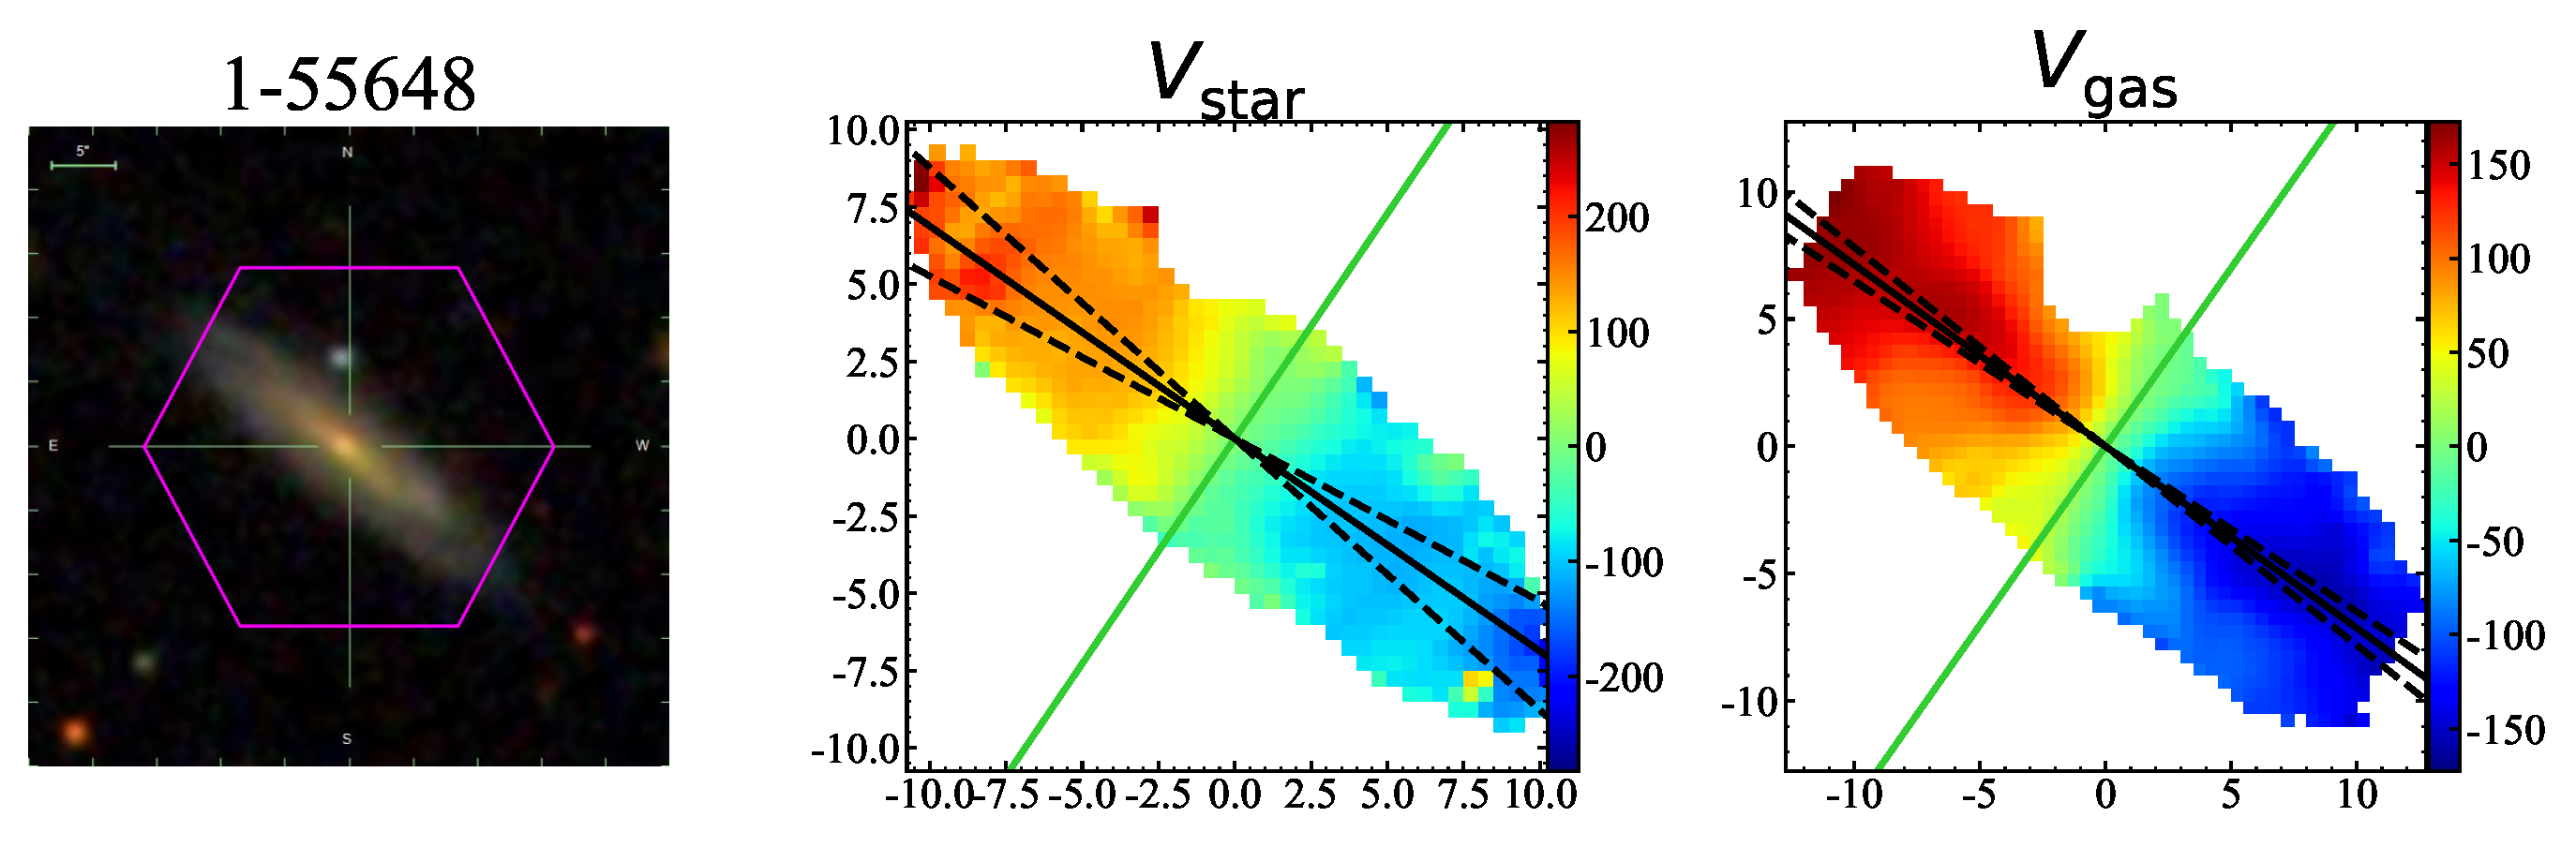
\includegraphics[width=2.0\columnwidth]{pics/explain_PA/PA_1-55648.eps}
    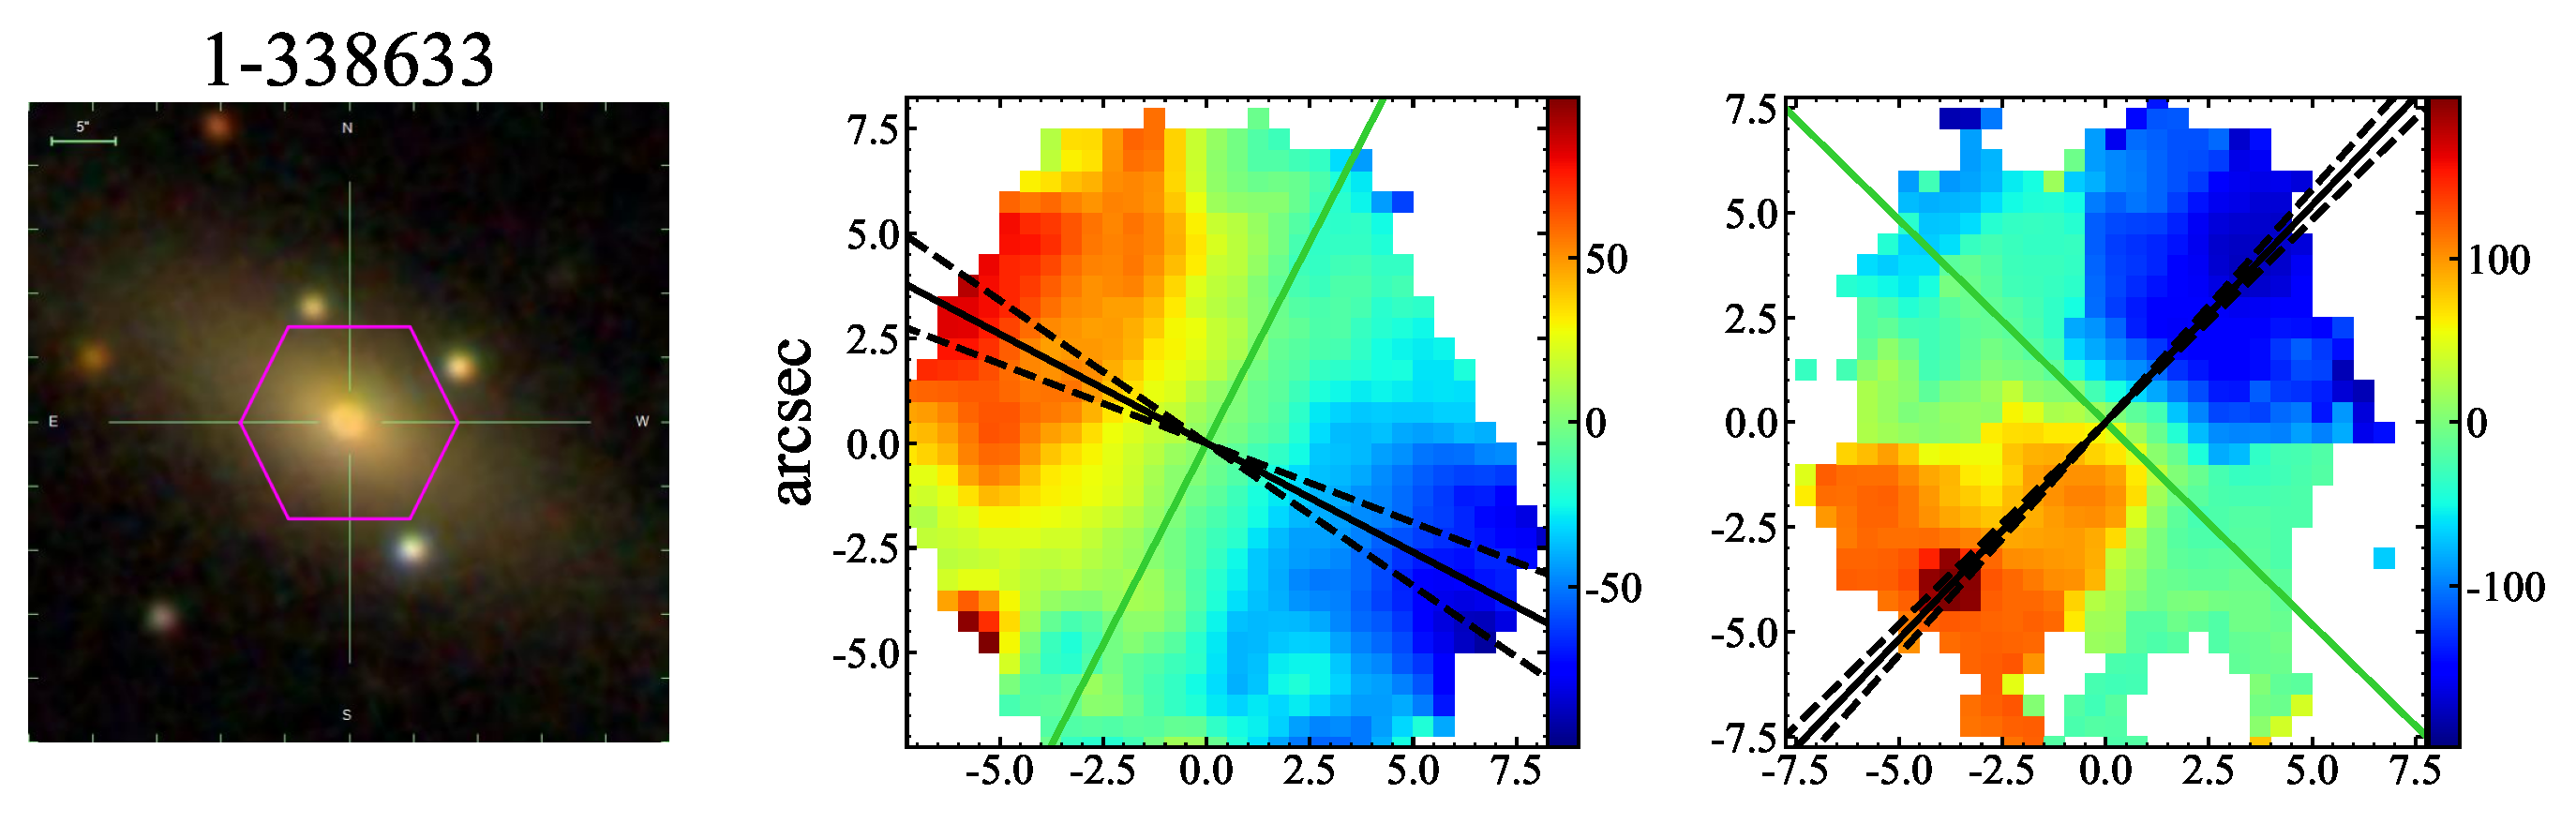
\includegraphics[width=2.0\columnwidth]{pics/explain_PA/PA_1-338633.eps}
    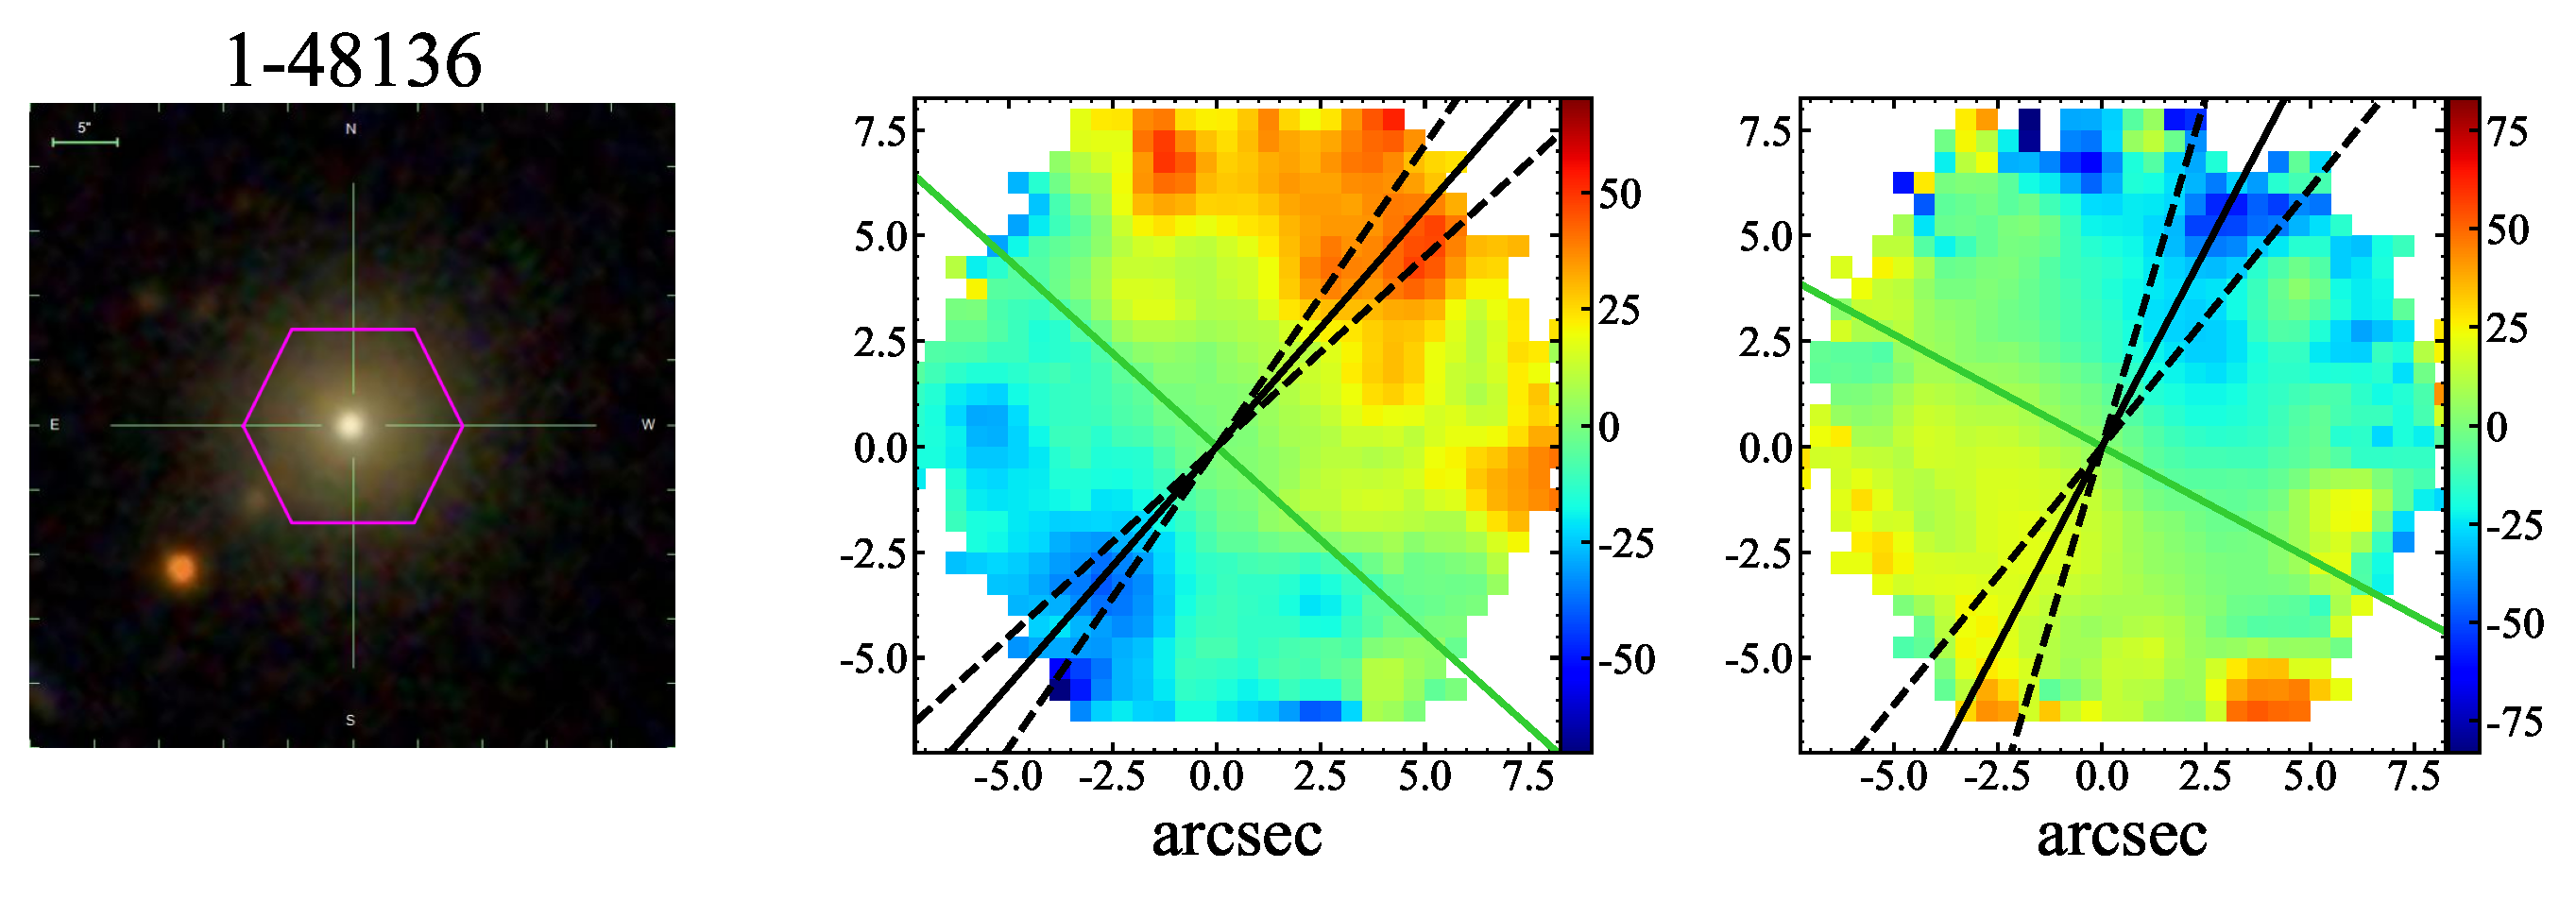
\includegraphics[width=2.0\columnwidth]{pics/explain_PA/PA_1-48136.eps}
    \caption{Examples of three MaNGA galaxies. Each row represents a galaxy (MaNGA ID is shown on the top). The left panel shows the SDSS \textit{g,r,i}-band image, the middle panel shows the stellar velocity field and the right panel shows the gas velocity field. The rotation velocities are indicated by the color bar, the red side is moving away from us while the blue side is approaching us. The solid black lines and green lines in each velocity field show the major and minor axis of the velocity field fitted by Python module FIT\_KINEMATIC\_PA \citep{krajnovic_kinemetry_2006}, while two dashed lines show $\pm 1 \sigma$ error range of PAs. The top row shows a galaxy (MaNGAID 1-55648) that has kinematically aligned stars and gas with $\Delta$PA $= 1^{\circ}$; the middle row shows a galaxy (MaNGAID 1-338633) with gas and stars rotating perpendicularly with $\Delta$PA $= 74^{\circ}$; the bottom row shows a galaxy (MaNGAID 1-48136) with gas and stars counter-rotating with $\Delta$PA $= 167^{\circ}$.}
    \label{fig:explain_PA}
\end{figure*}

In this paper, we select 460 gas-star misaligned galaxies from the internal Product Launch-10 (MPL-10) in Mapping Nearby Galaxies at Apache Point Observatory \citep[MaNGA,][]{2015ApJ...798....7B}, a new internal field spectroscopic survey. As a follow-up work of \cite{jin_sdss-iv_2016}, the sample size is enlarged by a factor of 7. Based on this largest misaligned sample so far, we look into the properties (i.e. kinematics, stellar populations, star formation activities, gas-phase metallicities) of these misaligned galaxies. The paper is organized as follows, In Section \ref{sec:data}, we present the selection of misaligned galaxies and their control samples. In Section \ref{sec:data analysis}, we compare the spatial resolved properties between misaligned galaxies and the control samples. We discuss the observational results in Section \ref{sec:discussion}. In Section \ref{sec:conclusions}, we briefly summarize the results. Throughout this paper, we adopt a flat $\Lambda$CDM cosmology with $\Omega_\Lambda=0.7$, $\Omega_{\rm m}=0.3$, and $H_0=70$ km s$^{-1}$ Mpc$^{-1}$.


\section{data}
\label{sec:data}

\subsection{The MaNGA survey}

MaNGA is one of the three core programs in the fourth-generation Sloan Digital Sky Survey (SDSS-IV) which began on July, 2014 \citep{2015ApJ...798....7B, drory_manga_2015}, it employs the Baryon Oscillation Spectroscopic Survey (BOSS) spectrographs \citep{smee_multi-object_2013} on the 2.5m Sloan Foundation Telescope \citep{gunn_25_2006}. The MaNGA observing strategy is described in \citet{law_observing_2015}, the MaNGA data proc pipeline is described in \citet{law_data_2016} and the flux calibration scheme is presented in \citet{yan_sdss-ivmanga_2016}. An overview of the survey execution strategy and data quality is provided in \citet{yan_sdss-iv_2016}. MaNGA has finished the survey of an unprecedented sample of $\sim$10,000 nearby galaxies early 2021 with a flat distribution in stellar masses in between $9 \le {\rm log}(M_*/M_\odot) \le 11$, the full redshift range is 0.01 $< z <$ 0.15 with a median value of $z \sim$ 0.03 \citep{2017AJ....154...86W, blanton_sloan_2017}. MaNGA employs dithered observations with 17 hexagonal integral field units (IFU) that vary in diameter from 12\arcsec (19 fibers) to 32\arcsec (127 fibers). Two dual-channel spectrographs provide simultaneous wavelength coverage over 3600$-$10,300 \r{A} with a median resolution $R \sim$ 2000. The typical spatial resolution is 1$\sim$2 kpc. The target galaxies are divided into "primary" and "secondary" sample following a ratio of 3 : 1. The primary sample is resolved out to $\sim$1.5 effective radius ($R_{\rm e}$, Petrosian 50\% light radius) while the secondary sample is observed to $\sim$2.5 $R_{\rm e}$. A total exposure time of 3 hours on-sky ensures a per-fiber \textit{r}-band continuum signal-to-noise ratio (S/N) per pixel of roughly 5 in the outskirts of target galaxies, with much higher S/N towards the center.

\subsection{Sample of kinematically misaligned galaxies}
\label{sec:Sample of kinematically misaligned galaxies}

\begin{figure}
    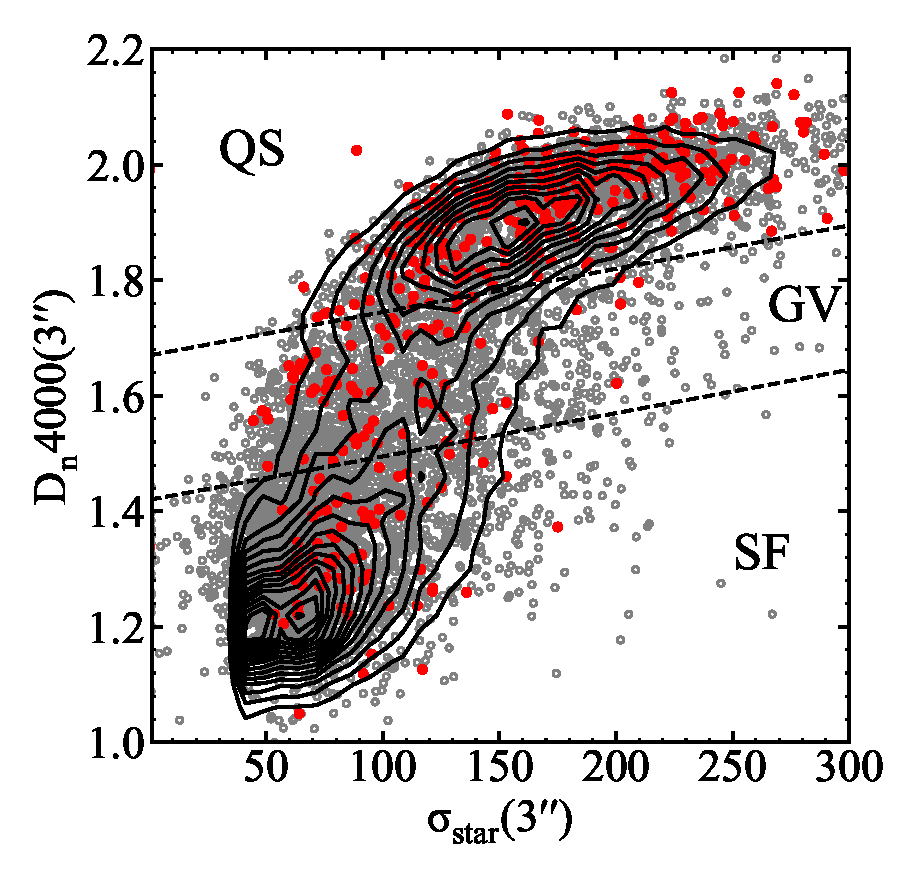
\includegraphics[width=\columnwidth]{pics/contour_Dn4000_V_DISP_3arcsec-3arcsec.eps}
    \caption{Diagram of central $3^{\prime \prime}$ D$_n$4000 versus ${\sigma}_{\rm star}$ for misaligned galaxies (red dots) and MaNGA sample (grey circles), with the SDSS DR7 sample shown as contours. There are two number density peaks in the contour. The two black dashed lines separate galaxies into star forming, green valley and quiescent sequence galaxies. The top dashed line is an approximation of the lower boundary of star forming main sequence (at the $\sim$1$\sigma$ level in scatter), while the bottom dashed line is an approximation of the upper boundary of quiescent sequence.}
    \label{fig:contour_Dn4000_V_DISP_3arcsec-3arcsec}
\end{figure}

\begin{table}
    \caption{Classification result of aligned/misaligned galaxies.}
    \label{tab:classification result}
    \begin{tabular}{lcc}
        \hline
        Aligned/Misaligned & Type & Number \\
        \hline
        Aligned & & 6502\\
        Misaligned & & \\
         & SF & 72\\
         & GV & 142\\
         & QS & 242\\
        Total & & 6958\\
        \hline
    \end{tabular}
\end{table}

\begin{figure}
    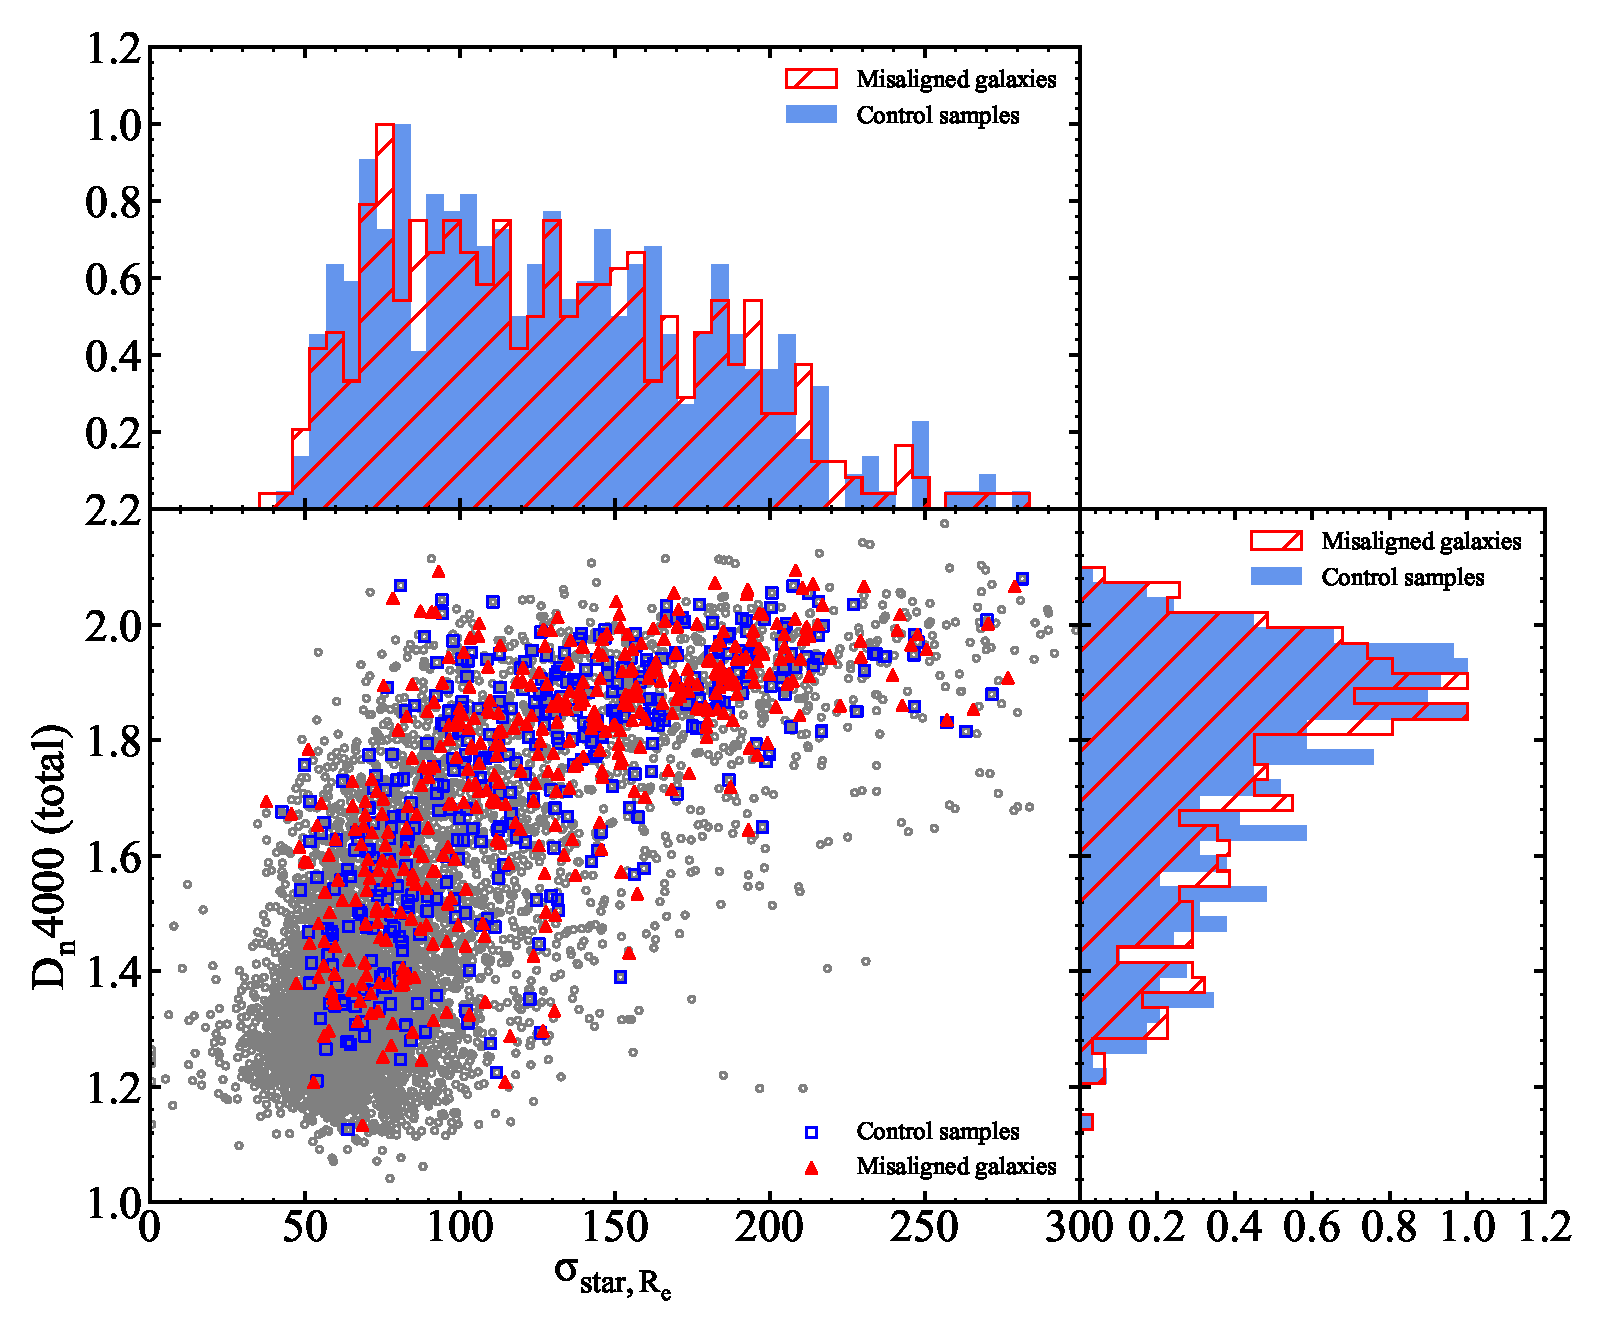
\includegraphics[width=1.0\columnwidth]{pics/Dn4000_sigma.eps}
    \caption{Total D$_n$4000 versus $\sigma_{{\rm star}, R_{\rm e}}$ for misaligned galaxies (red triangles) and one control sample (blue squares). The MaNGA galaxies are shown as grey circles. The top and right histograms show distribution of $\sigma_{{\rm star}, R_{\rm e}}$ and D$_n$4000, respectively. In each panel, the histograms filled with red lines are for the kinematically misaligned galaxies and that filled with blue color are for the control sample. The peaks of the distributions are set to 1.0.}
    \label{fig:Dn4000_sigma_star}
\end{figure}

The MaNGA sample and data products used in this work are drawn from the internal MaNGA Product Launch-10 (MPL-10), which includes 9456 unique galaxies. The MaNGA data analysis pipeline \citep[DAP,][]{westfall2019data} uses pPXF \citep{cappellari2004parametric} and a subset of stellar templates  from MaSTar library \citep{yan_sdss-iv_2019} to fit the stellar continuum in each spaxel. The data products include estimation of the stellar absorption and measurements of 21 major nebular emission lines in 3600$-$10,300 \r{A}, emission line fluxes are corrected for underlying stellar continuum absorption. The parameters we extracted from MaNGA DAP products named as "SPX-GAU-MILESCH-MASTARHC2", including : line-of-sight rotation velocity of stars ($V_{\rm star}$), stellar velocity dispersion (${\sigma}_{\rm star}$), line-of-sight rotation velocity of ionized gas ($V_{\rm gas}$), gas velocity dispersion (${\sigma}_{\rm gas}$), emission line fluxes (e.g. $\oiii\lambda$5007, $\ha$), lick indexes such as D$_n$4000, which is defined as the flux ratio between two narrow bands of 3850$-$3950 and 4000$-$4000 \r{A}.

In order to quantify the kinematic misalignment between stellar and gas components, we require the galaxies to have robust measurements of emission lines. We first separate the MaNGA sample into emission line galaxies and "line-less" galaxies."line-less" galaxies are defined as galaxies with $\ha$ signal-to-noise ratio smaller than 3 for more than $90\%$ spaxels within $\sim$1.5 $R_{\rm e}$. For 6958 emission line galaxies, we fit the kinematic position angle (PA) to both stellar (${\rm PA}_{\rm star}$) and gas (${\rm PA}_{\rm gas}$) velocity fields. The kinematic PA is measured based on established methods of \citet{krajnovic_kinemetry_2006}, it is defined as the counter-clockwise angle between north and a line that bisects the velocity field of gas or stars, measured on the receding side.

In Fig.~\ref{fig:explain_PA}, we show three examples of MaNGA galaxies. Each row represents a galaxy. The left panel shows the SDSS \textit{g,r,i}-band image (MaNGA ID is shown on the top), the middle panel shows the stellar velocity field and the right panel shows the velocity field of ionized gas traced by $\ha$. The values of rotation velocities are indicated by the color bar, the red side is moving away from us while the blue side is approaching us. The solid black and green lines in each velocity field show the kinematic major and minor axis fitted by Python module FIT\_KINEMATIC\_PA \citep{krajnovic_kinemetry_2006}, while two dashed lines show $\pm1\sigma$ error range. The top row shows a galaxy that has kinematically aligned gas and stellar components with $\Delta$PA = $1^{\circ}$; the middle row shows a galaxy with gas and stars rotating perpendicularly with $\Delta$PA $= 76^{\circ}$; the bottom row shows a counter-rotating galaxy with $\Delta$PA $= 167^{\circ}$. We identify 723 galaxies with robust PA measurement (error of PA < $60^{\circ}$) and $\Delta$PA $\ge 30^{\circ}$ as our kinematic decoupled sample. We eyeball both the photometry and velocity fields of these galaxies, removing irregular galaxies, broad line AGNs and on-going mergers. Finally the sample size is reduced to 456 galaxies.

Fig.~\ref{fig:contour_Dn4000_V_DISP_3arcsec-3arcsec} shows D$_n$4000-${\sigma}_{\rm star}$ relation for the central $3^{\prime \prime}$ of misaligned galaxies (red dots) and MaNGA galaxy sample (grey circles), with the SDSS DR7 sample shown as contours. The value of D$_n$4000 and ${\sigma}_{\rm star}$ within $3^{\prime \prime}$ are taken from MPA/JHU catalogue\footnote{https://wwwmpa.mpa-garching.mpg.de/SDSS/DR7/}. There are two density peaks in the contour. The peak at the bottom-left with lower D$_n$4000 and $\sigma_{\rm star}$ corresponds to younger stellar population, we refer them as star-forming (SF), the peak at the top-right with higher D$_n$4000 and $\sigma_{\rm star}$ corresponds to older stellar population, we refer them as quiescent sequence (QS). The population in between SF and QS is referred as green-valley (GV). The two black dashed lines separate these three populations. The top dashed line is an approximation of the lower boundary of star forming main sequence (at the $\sim$1$\sigma$ level in scatter), while the bottom dashed line is an approximation of the upper boundary of quiescent sequence. The classification result is listed in Table.~\ref{tab:classification result}. The reason that we do not apply the widely used SFR-$M_*$ relation to separate SF, GV, QS populations, includes: (1) different from SFR, D$_n$4000 can be measured consistently for all galaxies \citep{chen_post-starburst_2019}; (2) we hope to avoid any potential influence on the measurement of emission line strength due to the interaction between pre-existing and accreted external gas; (3) we find the median stellar velocity dispersion of the misaligned samples is 20$\sim$30 km$\rm \, s^{-1}$ larger than a control sample with similar D$_n$4000 and stellar mass distribution, considering that $\sigma_{\rm star}$ is a direct observed property that reflects the depth of the potential well of a galaxy \citep{2000ApJ...539L...9F, gebhardt2000relationship}, we use $\sigma_{\rm star}$ instead of $M_*$ in this work.

\subsection{Control sample}

It is believed that the gas components in the kinematically misaligned galaxies primarily originate from external processes like mergers and gas accretion. In order to understand the influence of external gas acquisition on the evolution of galaxies, we build control sample of galaxies with $\Delta$PA $< 30^{\circ}$. For each misaligned galaxy, we find ten non-misaligned galaxies which are closely matched in $\sigma_{{\rm star}, R_{\rm e}}$ ($|\Delta{\sigma}_{{\rm star}, R_{\rm e}}| \leq 8$) and global D$_n$4000 ($|\Delta$D$_n$4000$| \leq 0.05$) to construct the control sample. $\sigma_{{\rm star}, R_{\rm e}}$ is the stellar velocity dispersion at $R_{\rm e}$. Global D$_n$4000 is measured from the global spectrum within MaNGA bundle.

Fig.~\ref{fig:Dn4000_sigma_star} shows the misaligned sample (red triangles) and the control sample (blue squares) on the total D$_n$4000 versus $\sigma_{{\rm star}, R_{\rm e}}$ plane. The top and right histograms show distribution on $\sigma_{{\rm star}, R_{\rm e}}$ and D$_n$4000, respectively. It is clear that misaligned galaxies and control sample have the same distribution on $\sigma_{{\rm star}, R_{\rm e}}$ and total D$_n$4000.

Through quantifying the difference between the misaligned galaxies and the control sample, our aim is to have an idea about how the external processes influence galaxies evolution. 


\section{data analysis}
\label{sec:data analysis}

\begin{figure*}
    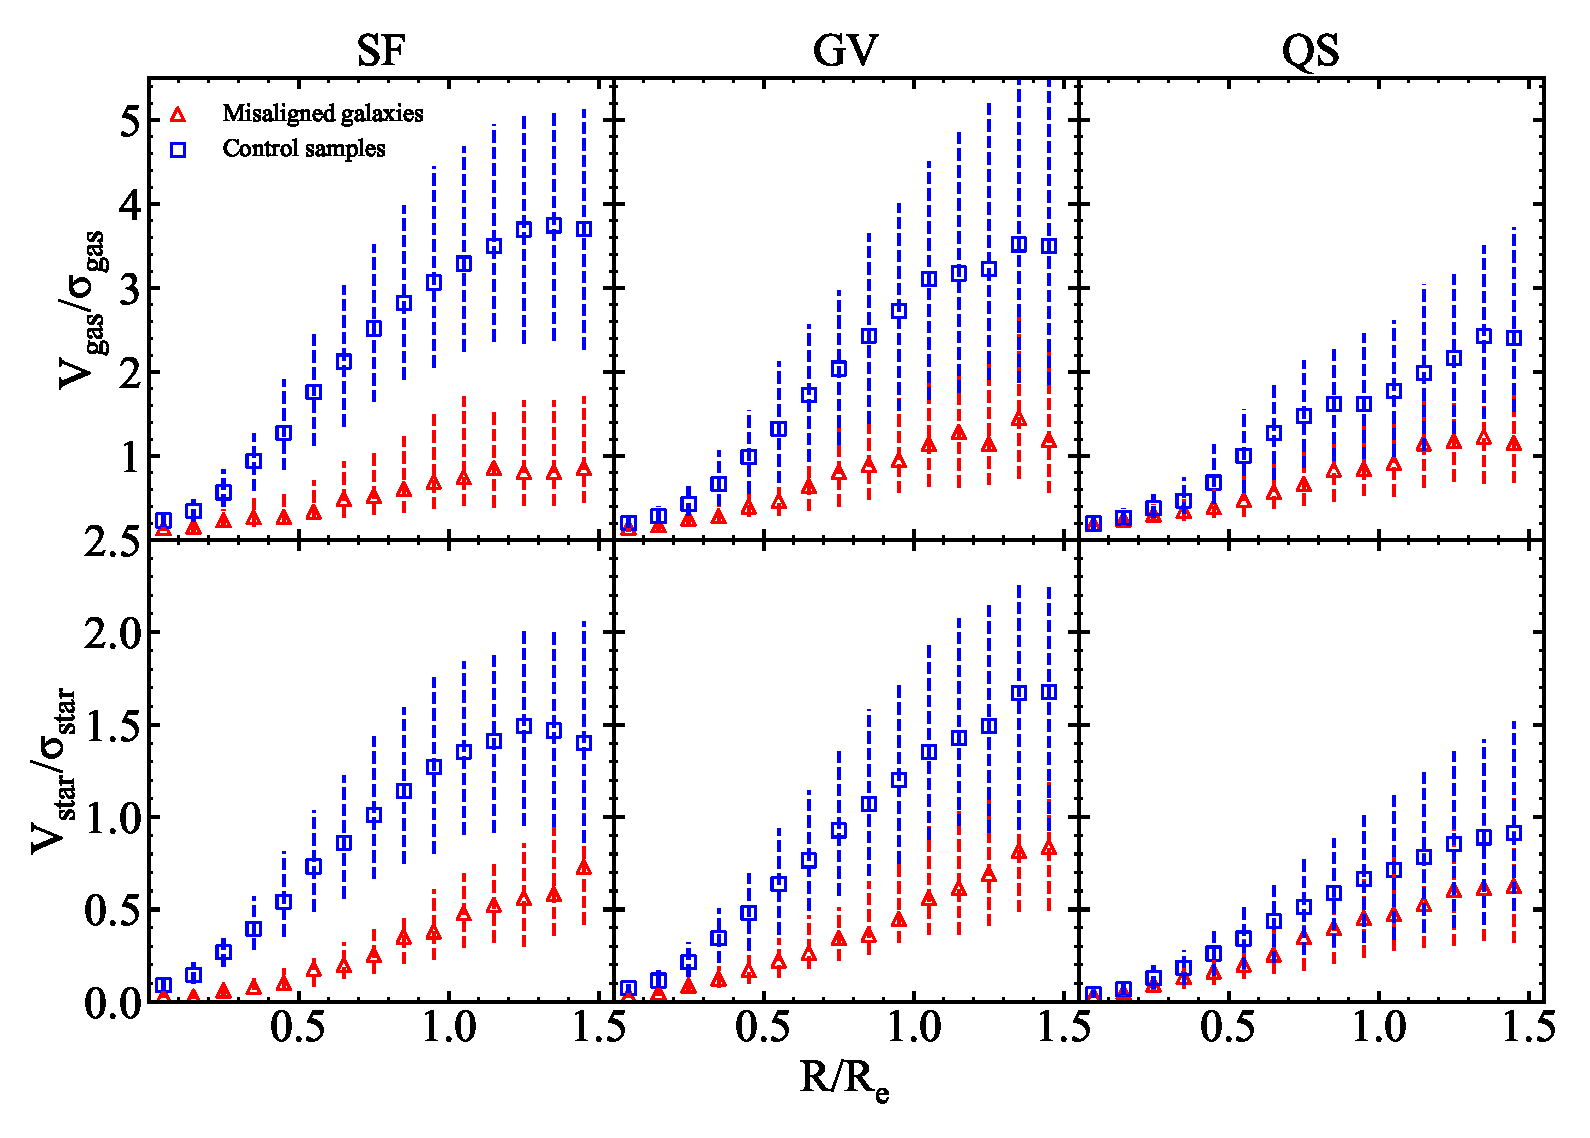
\includegraphics[width=2.0\columnwidth]{pics/vel_divide_sigma_gas_stellar.eps}
    \caption{Comparison of ${\rm V}_{\rm gas}/{\sigma}_{\rm gas}$ (top row) and ${\rm V}_{\rm star}/{\sigma}_{\rm star}$ (bottom row) radial profiles within 1.5 ${\rm R}_{\rm e}$ between misaligned galaxies and control sample. The left panel is for SF, the middle panel is for GV, the right panel is for QS. The red triangles represent the median value of misaligned galaxies and the blue squares represent the median value of control sample. The error bars show the 30th and 70th percentiles of the distribution. The radii are the projected distances from the galactic centre to the spaxels where indices are measured in the unit of the effective radius.}
    \label{fig:vel_divide_sigma}
\end{figure*}

\begin{figure*}
    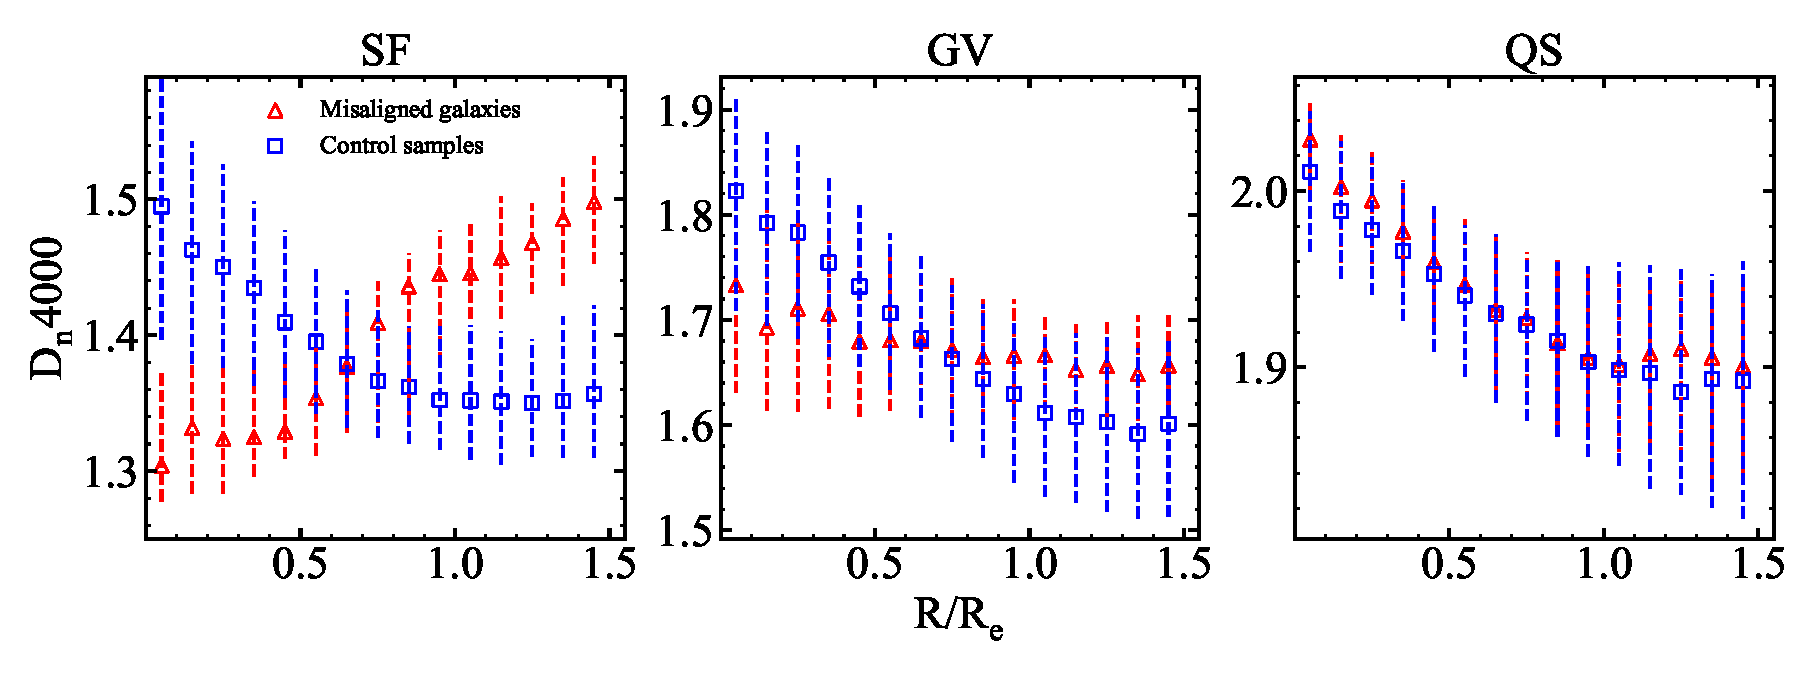
\includegraphics[width=2.0\columnwidth]{pics/Dn_4000.eps}
    \caption{Comparison of D$_n$4000 radial profiles within 1.5 $R_{\rm e}$ between misaligned galaxies and control sample. Red triangles represent misaligned galaxies and blue squares represent control sample.}
    \label{fig:Dn(4000)}
\end{figure*}

In this section, we compare the spatial resolved properties between the misaligned galaxies and their control sample, including the average gas and stellar velocity to velocity dispersion ratio ($V_{\rm gas}/{\sigma}_{\rm gas}$ and $V_{\rm star}/{\sigma}_{\rm star}$), stellar population (D$_n$4000, light and mass-weighted stellar age, on going star forming rate), gas-phase metallicity. We hope to have a picture about the evolution of the misaligned galaxies through this section.

\subsection{Kinematics}

The ratio between ordered to random stellar motion in galaxies is strongly depending on luminosity and stellar mass \citep{veale_massive_2017, green_sami_2018}, which indicates a link between the build-up of stellar mass and angular momentum over cosmic time, which is fundamental in understanding the large variations in morphology and star formation in present-day galaxies. Major mergers are primary candidates for a dramatic changing in the morphology and spin of galaxies, however merger is only one of the many physical processes at play over the lifetime of a galaxy, continuing gas accretion and star formation can reshape the morphology and kinematics of remnants \citep{naab_atlas3d_2014}. In this section, we compare the ratio of radial gradients of velocity to velocity dispersion of gas and stellar components, $V_{\rm gas}/{\sigma}_{\rm gas}$ and $V_{\rm star}/{\sigma}_{\rm star}$, try to discern any difference in the formation/interaction history of the misaligned and control sample.

Fig.~\ref{fig:vel_divide_sigma} shows the median velocity to velocity dispersion ratio for gas and stellar components, $V_{\rm gas}/{\sigma}_{\rm gas}$ (top row) and $V_{\rm star}/{\sigma}_{\rm star}$ (bottom row), along their kinematic major axis for the misaligned sample and the control sample. In each row, the left panel is for SF, the middle panel is for GV and the right panel is for QS. The red triangles represent the median value of the misaligned sample and the blue squares represent the median value of the control sample. The error bars show the 30th and 70th percentiles of the distribution. The larger (smaller) value of $V/\sigma$ corresponds to more (less) rotationally support for the relevant components. $V$/$\sigma$ are taken from MaNGA DAP files, they are estimated from the spectral fitting process described in Sec.~\ref{sec:Sample of kinematically misaligned galaxies}. We can find that SF, GV, QS misaligned galaxies have $V_{\rm gas}/{\sigma}_{\rm gas}$ and $V_{\rm star}/{\sigma}_{\rm star}$ smaller and systematically shifted than their control samples. The difference between misaligned galaxies and control samples in QS is much smaller than that in SF and GV, indicating that external gas accretion has larger influence on the evolution (morphology) of SF, GV galaxies than QS galaxies.

\citet{chen_growth_2016} and \citet{jin_sdss-iv_2016} find that the central regions of star-forming misaligned galaxies show more intense, ongoing star formation and younger stellar populations than their outskirts, suggesting these galaxies accrete abundant external gas, the interaction between accreted and pre-existing gas triggers gas into central regions and forms new stars. The lower value of $V_{\rm star}/{\sigma}_{\rm star}$ and $V_{\rm gas}/{\sigma}_{\rm gas}$ in the star-forming misaligned galaxies than their controls can be easily understood under this picture in the following way: the interaction between accreted external gas and pre-existing gas (in the extreme case, they are counter-rotating) leads to the cancellation of angular momentum, thus lowers $V_{\rm gas}/{\sigma}_{\rm gas}$ as well as $V_{\rm star}/{\sigma}_{\rm star}$ once the gas transforms into stars. 

The GV and QS misaligned galaxies appear to have been undergoing a similar process to that seen in the star-forming misaligned galaxies which lead to the lower value of $V_{\rm star}/{\sigma}_{\rm star}$ and $V_{\rm gas}/{\sigma}_{\rm gas}$ than the control sample, but, on the one hand, the gas accretion and trigger of star formation happened earlier; on the other hand, the process is less violent in QS galaxies since the amount of both pre-existing and accreted gas is small in QS galaxies.

\begin{figure*}
    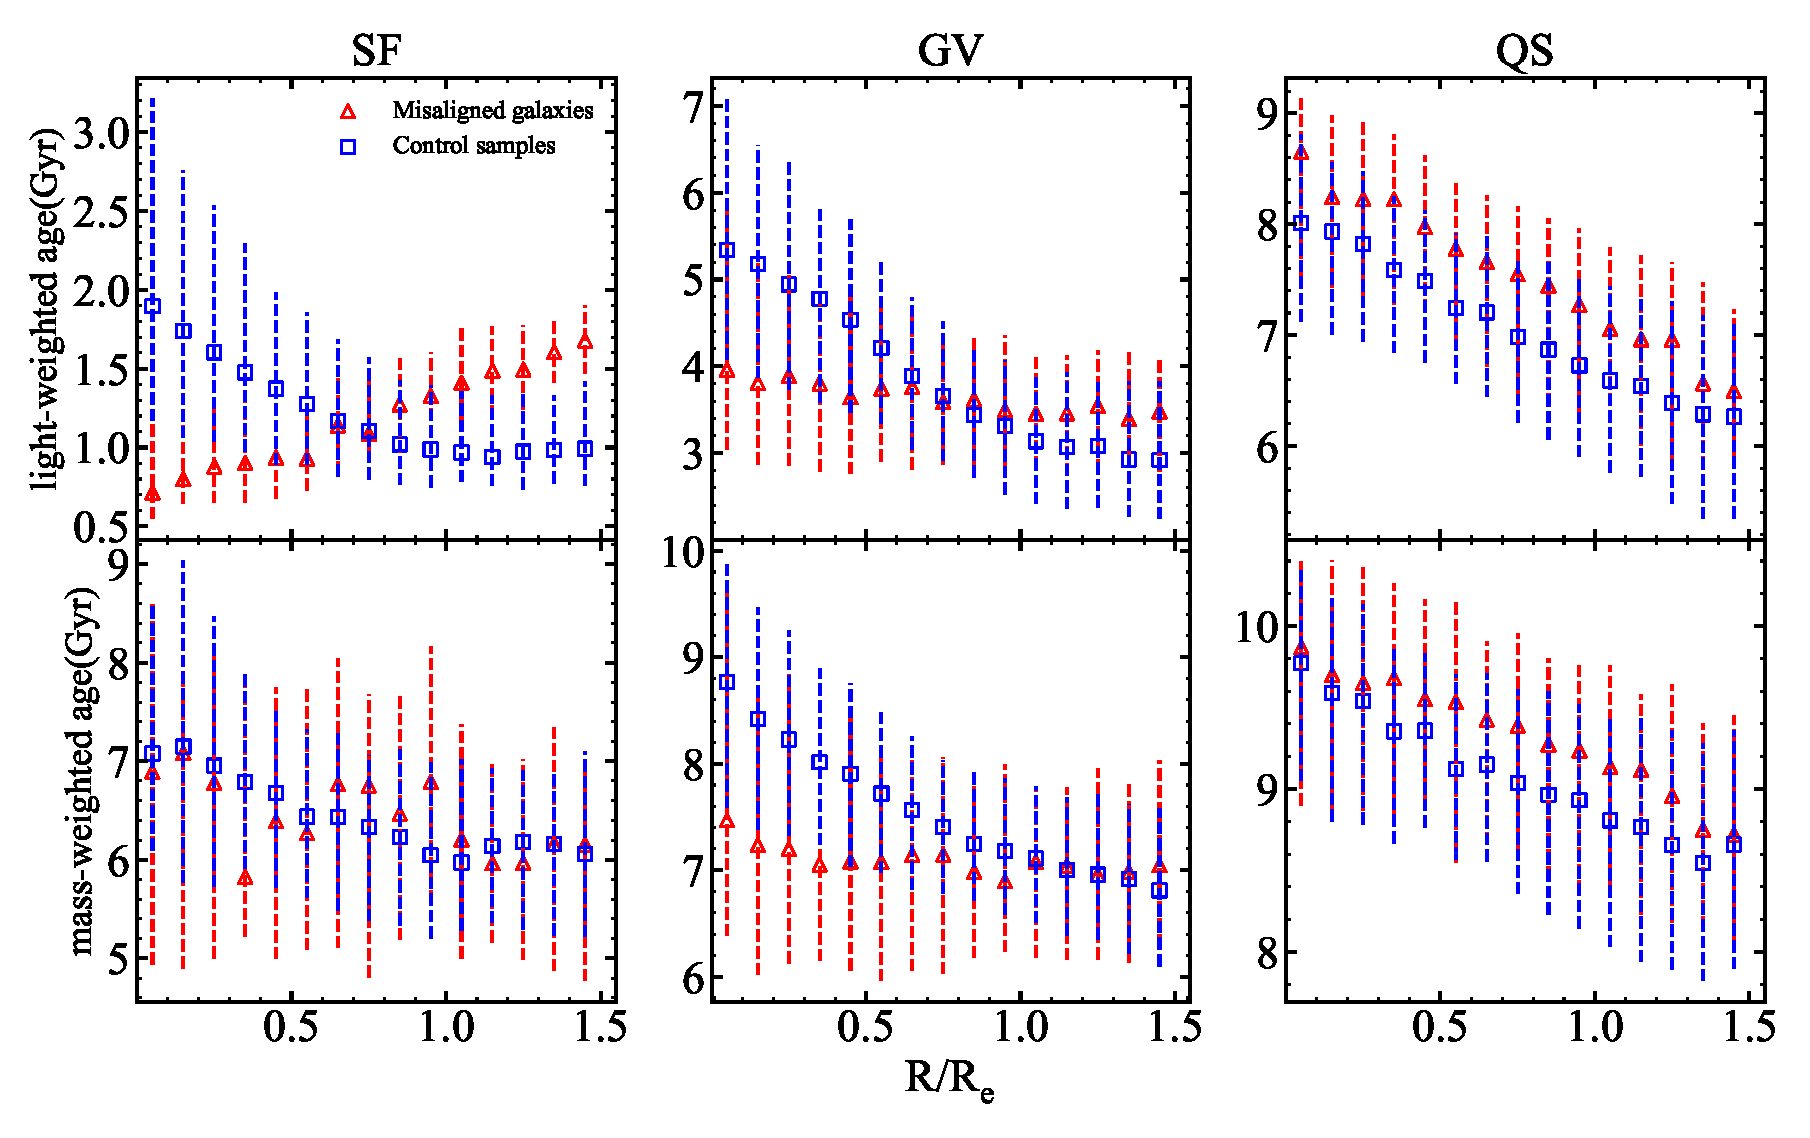
\includegraphics[width=2.0\columnwidth]{pics/lw_age_and_mw_age.eps}
    \caption{Comparison of light-weighted stellar ages and mass-weighted stellar age radial profiles within 1.5 $R_{\rm e}$ between misaligned galaxies and control sample. Red triangles represent misaligned galaxies and blue squares represent control sample.}
    \label{fig:lw_age_and_mw_age}
\end{figure*}

\begin{figure*}
    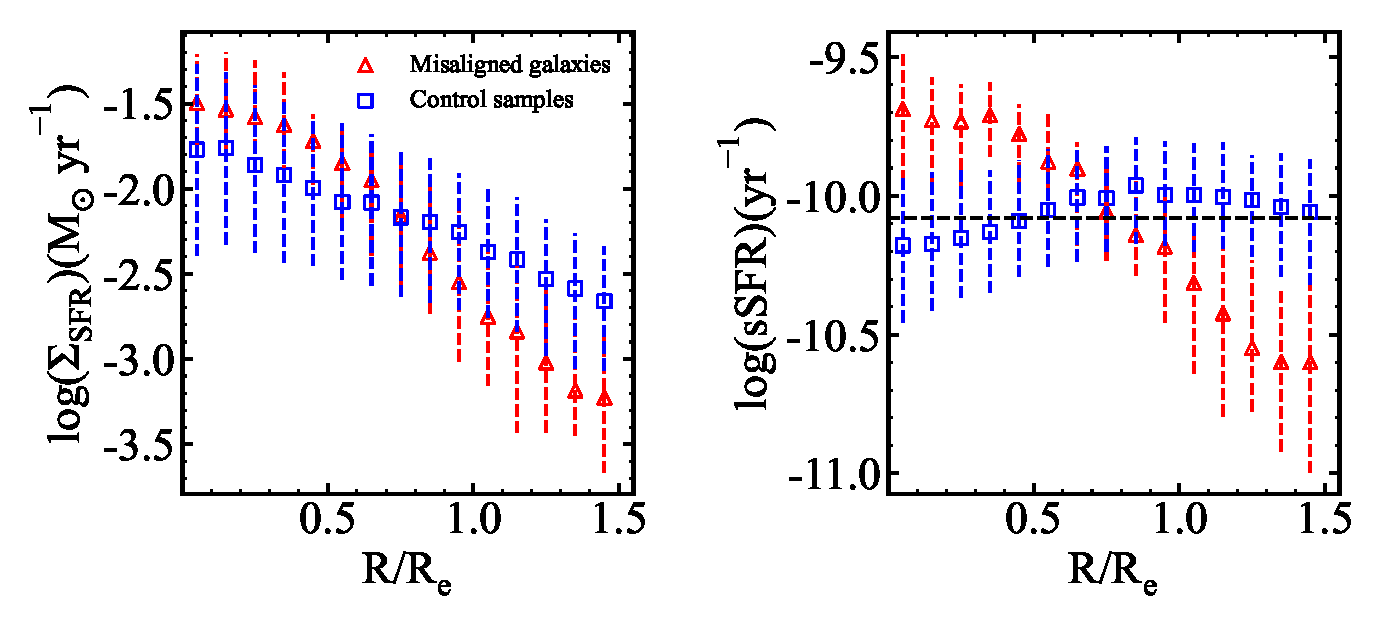
\includegraphics[width=1.6\columnwidth]{pics/SFR_and_sSFR.eps}
    \caption{Comparison of star formation rate surface density and specific star formation rate radial profiles within 1.5 $R_{\rm e}$ between SF misaligned galaxies and control sample. Red triangles represent misaligned galaxies and blue squares represent control sample. The horizontal dashed line is defined as 1/($t_{\rm{H}(z)}-1\,\rm Gyr$), where $t_{\rm{H}(z)}$ is the Hubble time at the median redshift of the MaNGA star forming galaxy sample.}
    \label{fig:SFR_and_sSFR}
\end{figure*}

\subsection{Stellar population}

In this section, we study the stellar population distribution of the misaligned galaxies and control sample using continuum spectral indices D$_n$4000, light-weighted stellar age and mass-weighted stellar age as well as the ongoing star formation rate. 

Fig.~\ref{fig:Dn(4000)} shows the D$_n$4000 radial profiles for the SF (left), GV (middle) and QS (right) galaxies. Again, red triangles represent misaligned galaxies and blue squares represent control sample. For the star-forming galaxies, the D$_n$4000 gradient of misaligned galaxies is positive while the gradient of control sample is negative. At $R$ < $\sim$0.7 $R_{\rm e}$, the median value of D$_n$4000 is lower (younger in stellar population) for the misaligned galaxies than the control sample. Over this radius, the result is totally inverse, the stellar population in misaligned galaxies becomes older (higher D$_n$4000) than the control galaxies. This is consistent with the results in \citet{chen_growth_2016}, \citet{jin_sdss-iv_2016} and \citet{bizyaev_sdss_2019}, indicating that SF misaligned galaxies have younger stellar population in the centre than that in the outskirts. The explanation for this outside-in growth mode in SF misaligned galaxies is that the redistribution of angular momentum occurs from gas-gas collisions between the pre-existing and the accreted gas largely accelerates gas inflow, on the one hand leading to a fast centrally concentrated star formation, on the other hand shutting down the star formation in the outskirts due to the lack of cold gas. The controls have a negative gradient in D$_n$4000, indicating older stellar populations in the centre, as expected for ordinary bulge+disk structure of star-forming galaxies, consistent with the inside-out growth mode. For the GV misaligned galaxies (middle panel), the median D$_n$4000 has a flat distribution over radius, with a roughly constant value of 1.7, while control sample has a negative gradient in D$_n$4000. Similar to the SF galaxies, the stellar population is younger with lower D$_n$4000 in the misaligned galaxies than the control sample at $R$ < $\sim$0.7 $R_{\rm e}$, and older over this radius. This suggests that the GV galaxies was undergoing similar process after external gas accretion as the SF galaxies. The smaller difference in D$_n$4000 between GV misaligned galaxies and the control sample indicates that this process happened either earlier or less violent than SF galaxies. The misaligned QS and their control galaxies have identical negative D$_n$4000 gradients, indicating external gas accretion either happened much earlier than the SF and GV galaxies or the influence on stellar population is negligible. The difference in D$_n$4000 between the misaligned galaxies and control sample decreases from SF to QS.

Fig.~\ref{fig:lw_age_and_mw_age} shows radial profiles in light-weighted stellar age (top row) and mass-weighted stellar age (bottom row). The two ages are taken from the Pipe3D Value Added Catalog \citep{2016RMxAA..52...21S, 2016RMxAA..52..171S}, in which the stellar continuum is fitted as a linear combination of synthetic single stellar population (SSP) templates. Again red triangles represent misaligned galaxies and blue squares represent the control sample. Since D$_n$4000 is a good indicator of light-weighted age of a stellar population, the radial profiles of light-weighted age and D$_n$4000 are very similar. It enhances the difference between misaligned galaxies and control sample, which can be seen from the distinct difference of light-weighted age in QS while D$_n$4000 shows little difference in QS. Mass-weighted ages of the SF misaligned galaxies show an overall flat distribution of old stellar population along radius (6$\sim$7 Gyr), which is totally different from the positive gradient of the light-weighted ages. Similar to the SF misaligned galaxies, the mass-weighted age gradient of their control sample is very shallow, and has similar value to that of misaligned galaxies. This suggests the underlying stellar population of the star forming misaligned galaxies is similar to the control samples, the current central concentrated star formation is simply a recent burst on top of a dominant old population. The misaligned galaxies in GV have a median mass-weighted age of 7$\sim$8 Gyr across the whole galaxies. At $R$ < 0.7$\sim$0.8 $R_{\rm e}$, it is $\sim$1 Gyr younger than the control samples (middle panel of Fig.~\ref{fig:lw_age_and_mw_age}) and becomes consistent with the controls at outskirts. For the misaligned QS galaxies, we find that their mass weighted ages are consistent with the control samples over radius, there is weak evidence that the misaligned galaxies are a little bit older, we do not tend to explain this tiny difference considering that the error bar of mass-weighted age measurement is quite large.

We estimate star formation rate surface density ($\Sigma_{\rm SFR}$) of star forming regions from the dust extinction corrected $\ha$ luminosity \citep{salpeter_luminosity_1955, kennicutt_star_1998} : $\rm SFR(M_{\sun} \ yr^{-1}) = 7.9 \times 10^{-42} \ L_{\ha} (erg \ s^{-1})$. Dust extinction is calculated from Balmer decrement ($\ha$ and $\hb$ flux ratio) under Case B, the Galactic dust extinction curve from \citet{calzetti_dust_2001} is applied. 
The specific star formation rate (sSFR) is defined as SFR/$M_*$ for each spaxel.

Fig.~\ref{fig:SFR_and_sSFR} shows radial profiles of the star formation rate surface density (left panel) and specific star formation rate (right panel) for SF galaxies. Again red triangles represent misaligned galaxies and blue squares represent the control samples. We only calculated $\Sigma_{\rm SFR}$ and sSFR for SF galaxies since there are very few star forming spaxels in GV and QS galaxies. As we can see, misaligned galaxies have higher $\Sigma_{\rm SFR}$ and sSFR within 0.7$\sim$0.8 $R_{\rm e}$ than their control sample, indicating that misaligned galaxies have enhanced recent star forming activity in the central regions. The horizontal dashed line in the right panel of Fig.~\ref{fig:SFR_and_sSFR} is defined as 1/($t_{\rm{H}(z)}-1\,\rm Gyr$), where $t_{\rm{H}(z)}$ is the Hubble time at the median redshift of the MaNGA star forming galaxy sample, and 1 Gyr is subtracted to account for the fact star formation primarily occurred after reionization. The higher sSFR for the central region of the misaligned sample than the value marked by the horizontal dashed line indicates that current SFR of the misaligned galaxies are higher than the past average ($M_*/(t_{\rm{H}(z)}-1\,\rm Gyr)$) of the local star forming galaxies, while the control sample have a current SFR which is similar to the past average, indicating fast growth of the central regions in the misaligned galaxies triggered by external gas accretion.

\subsection{Gas-phase metallicity}

\begin{figure*}
    
\includegraphics[width=2.0\columnwidth]{pics/metallicity.eps}
    \caption{Comparison of the radial profiles of gas-phase metallicities estimated from three different strong-line calibrators. Red triangles represent SF misaligned galaxies and blue squares represent the control samples. The left panel of Fig.~\ref{fig:metallicity} applies $R_{23}$ as the metallicity calibrator (Eq.1 in \citet{tremonti_origin_2004}), the middle panel applies O3N2 as the metallicity calibrator (Eq.2 in \citet{marino2013o3n2}), while N2S2\&N2$\ha$ is used in the right panel (Eq.2 in \citet{dopita_chemical_2016}). Red and blue crosses in left panel mark the median value of central $3^{\prime \prime}$ gas-phase metallicity from MPA-JHU catalogue for misaligned galaxies and control samples.}
    \label{fig:metallicity}
\end{figure*}

\begin{figure*}
    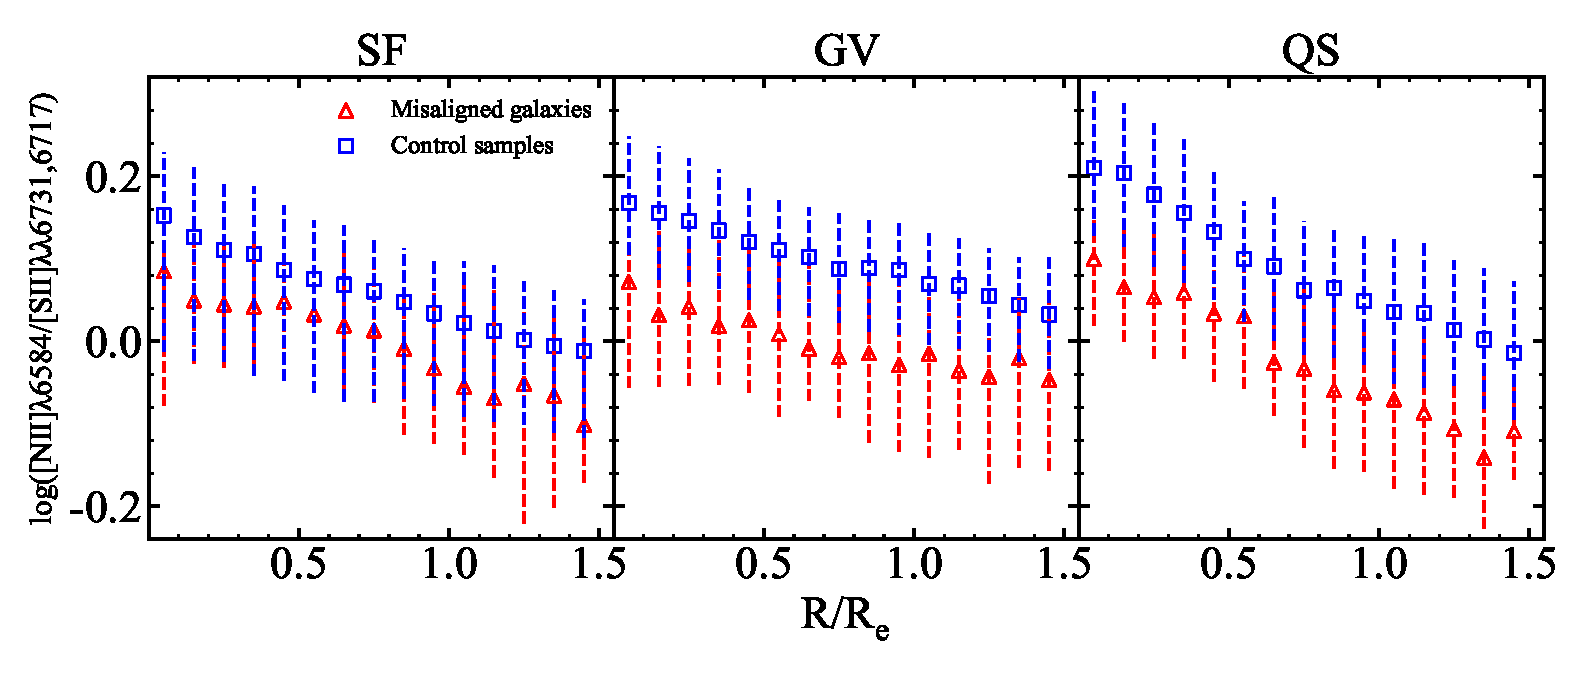
\includegraphics[width=2.0\columnwidth]{pics/NII_SII.eps}
    \caption{Comparison of {\nii}$\lambda$6584/{\sii}$\lambda\lambda$6717,6731 radial profiles within 1.5 $R_{\rm e}$ between misaligned galaxies and control sample. Red triangles represent misaligned galaxies and blue squares represent control sample.}
    \label{fig:NII_SII}
\end{figure*}

Gas-phase metallicity is one of the most fundamental physical properties of galaxies, it reflects the amount of gas reprocessed by stars and any exchange of gas between a galaxy and its environment.

The misaligned galaxies are believed to be the primary demonstrations whose evolution is regulated by external processes. External processes, such as minor/major mergers or gas accretion, could bring misaligned gas which has different metallicities from pre-existing gas into the galaxies. Thus, comparing the gas-phase metallicity between misaligned galaxies with their non-misaligned control sample will give us clues about the origin of misaligned gas as well as how the gas accretion processes influence the galaxy evolution.

Fig.~\ref{fig:metallicity} shows the radial profiles of gas-phase metallicity (estimated from three different strong line metallicity calibrators) for SF misaligned galaxies (red triangles) as well as their control samples (blue squares). The left panel of Fig.~\ref{fig:metallicity} applies $R_{23}$ as the metallicity calibrator (Eq.1 in \citet{tremonti_origin_2004}), the middle panel applies O3N2 as the metallicity calibrator (Eq.2 in \citet{marino2013o3n2}), while N2S2 and N2$\ha$ is used in the right panel (Eq.2 in \citet{dopita_chemical_2016}). Comparing the metallicities estimated from these three different calibrators, we find that although the absolute values and radial gradients of metallicity are different when we use different calibrators, they all point to the same conclusion that SF misaligned galaxies have overall lower gas-phase metallicity than their control samples. We do not discuss the difference in metallicities given by different calibrators in this work since unexpected systematic effect has been found by using different metallicity calibrators due to various reasons \citep{kewley_metallicity_2008, schaefer_sdss-iv_2019}.

Considering that the strong-line abundance diagnostics are developed based on the stellar population synthesis and photoionization models, it is limited to be only applied to $\hii$ regions \citep{kewley_using_2002}. However, the gas in the GV and QS galaxies is not excited by star formation for most of the spaxels, we thus follow \citet{jin_sdss-iv_2016} to apply $\nii\lambda6584/\sii\lambda\lambda6731,6717$ as an alternative gas-phase metallicity indicator. It is suggested by \citet{dopita_chemical_2016} and \citet{kashino2016hide} that $\nii\lambda6584/\sii\lambda\lambda6731,6717$ is a proxy for N/O ratio, and correlates with O/H abundance very well at 12 + log(O/H) $>$ 8.0. Also, the two emission lines are close in wavelength so the dust extinction correction is negligible. Fig.~\ref{fig:NII_SII} shows the radial gradients of $\nii\lambda6584/\sii\lambda\lambda6731,6717$ for the SF (left panel), GV (middle panel) and QS (right panel) misaligned galaxies (red triangles) as well as their control galaxies (blue squares). Similar to Fig.~\ref{fig:metallicity}, we find that the misaligned galaxies have lower gas-phase metallicities than their control samples, not only for the star forming galaxies, but also for green valley and quiescent galaxies, supporting the conclusion that the misaligned galaxies accreted low abundance gas from a gas-rich dwarf or cosmic web.

We have to point out that for the star forming misaligned galaxies, the difference in gas-phase metallicity between the misaligned galaxies and their controls strongly depends on how we define the control samples. We will discuss this in Section \ref{sec:discussion-1}.


\begin{figure*}
    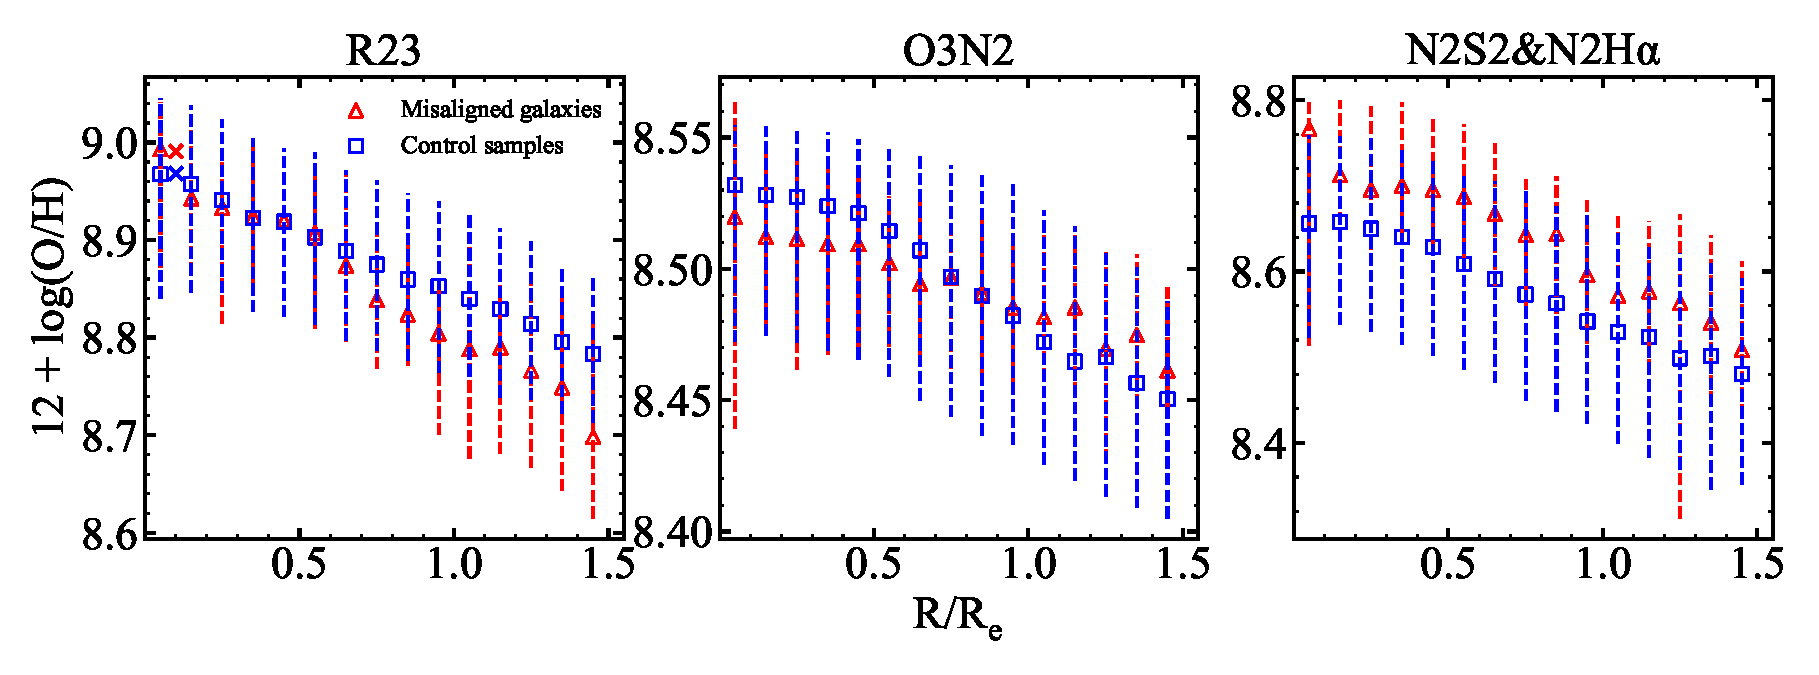
\includegraphics[width=2.0\columnwidth]{pics/SFR_M_control_sample/metallicity.eps}
    \caption{Comparison of gas-phase metallicities estimated from three different strong-line calibrators radial profiles within 1.5 $R_{\rm e}$ between misaligned galaxies and control sample closely matched in SFR and $M_*$. Same as Fig.~\ref{fig:metallicity}, but with the new control sample.}
    \label{fig:metallicity_SFR_M}
\end{figure*}

\begin{figure*}
    
\includegraphics[width=2.0\columnwidth]{pics/SFR_M_control_sample/NII_SII.eps}
    \caption{Comparison of {\nii}$\lambda$6584/{\sii}$\lambda\lambda$6717,6731 radial profiles within 1.5 $R_{\rm e}$ between misaligned galaxies and control sample closely matched in SFR and $M_*$. Same as Fig.~\ref{fig:NII_SII}, but with the new control sample.}
    \label{fig:NII_SII_SFR_M}
\end{figure*}

\begin{figure}
    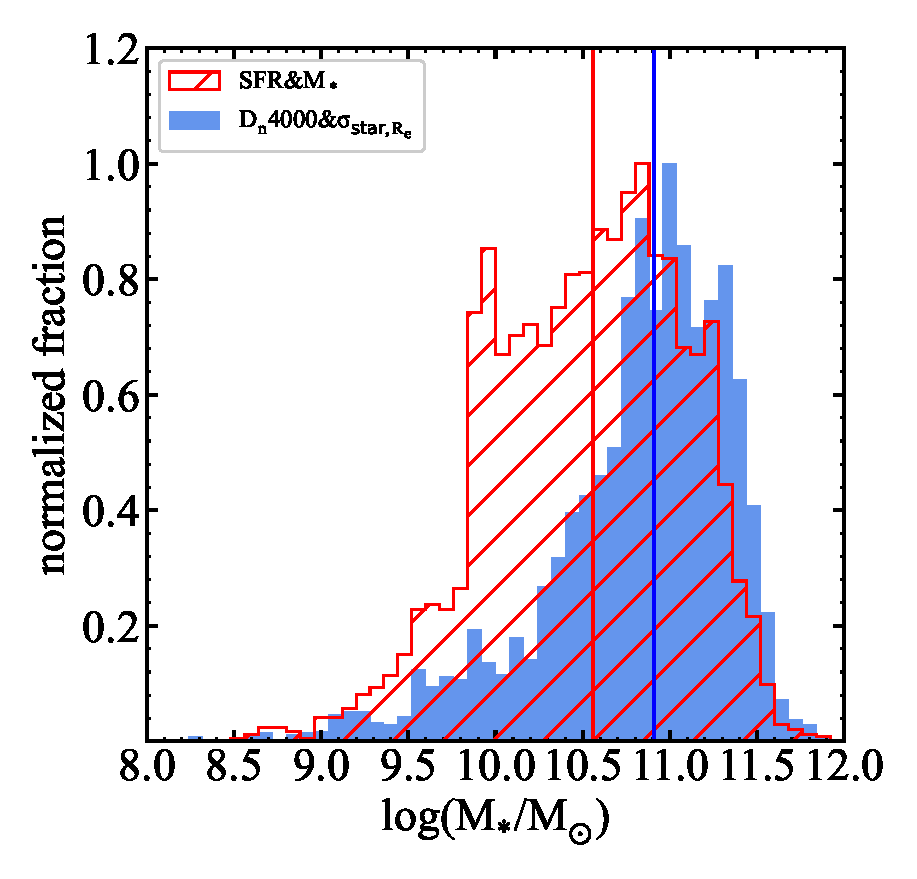
\includegraphics[width=1.0\columnwidth]{pics/SFR_M_control_sample/diff_M.eps}
    \caption{The $M_*$ distribution of control sample closely matched in SFR, $M_*$ (red histograms) as well as control sample closely matched in D$_n$4000, $\sigma_{{\rm star}, R_{\rm e}}$ (blue histograms). The red line is the median $M_*$ of control sample closely matched in SFR, $M_*$ while the blue line is the median $M_*$ of control sample closely matched in D$_n$4000, $\sigma_{{\rm star}, R_{\rm e}}$. The peaks of histogram are set to 1.0.}
    \label{fig:diff_M}
\end{figure}

\section{Discussion}
\label{sec:discussion}

Many previous works have studied the gas-star misalignment phenomena mostly in early type galaxies but rarely in star forming galaxies. Thanks to the large MaNGA sample, \citet{chen_growth_2016} and \citet{jin_sdss-iv_2016} detected gas-star misalignment in star forming galaxies. As a following work of \citet{jin_sdss-iv_2016}, we study the kinematics, stellar populations, star formation activities as well as metallicity of misaligned galaxies, and try to figure out the formation scenarios of misaligned galaxies, as well as how these mechanisms affect the properties of galaxies.

\subsection{Discrepancy in metallicity of SF misaligned galaxies}
\label{sec:discussion-1}
Our results on gas-phase metallicity of GV and QS misaligned galaxies are consistent with previous works \citep{chen_growth_2016, jin_sdss-iv_2016} that GV and QS misaligned galaxies have lower gas-phase metallicity than control samples. At first sight the result on gas-phase metallicity in SF misaligned galaxies seems contrary to previous works. \citet{chen_growth_2016} and \citet{jin_sdss-iv_2016} found SF misaligned galaxies have higher gas-phase metallicity than typical stellar mass-metallicity relation for local star-forming galaxies \citep{tremonti_origin_2004}, but this work finds SF misaligned galaxies have lower gas-phase metallicity than control samples. In this section, we focus on understanding the different results in gas-phase metallicity of SF misaligned galaxies and the dependance of our results on the selection of control samples.

We select another set of ten control samples that are closely match in SFR and $M_*$ with $|\Delta{\rm \log{SFR}}| \leq 0.2$ and $|\Delta{\log{M_*}}| \leq 0.1$, we repeat Fig.~\ref{fig:vel_divide_sigma} to Fig.~\ref{fig:NII_SII} based on the new control samples, finding that all the results are consistent with previous sections except the gas-phase metallicity of SF misaligned galaxies. Fig.~\ref{fig:metallicity_SFR_M} shows gas-phase metallicity estimated from three different strong-line calibrators for misaligned galaxies and the new control samples. The metallicity of the central region traced by $R_{23}$, N2S2\&N2$\ha$ and $\nii\lambda6584/\sii\lambda\lambda6731,6717$ is higher in misaligned galaxies than control samples, which is opposite to Fig.~\ref{fig:metallicity} and \ref{fig:NII_SII}. The central metallicity estimated from O3N2 of misaligned galaxies is still slightly lower than that of control sample. The red and blue crosses in the left panel of Fig.~\ref{fig:metallicity_SFR_M} mark the median value of central $3^{\prime \prime}$ gas-phase metallicity from MPA-JHU catalogue for misaligned galaxies and control samples. Our gas-phase metallicity in the central region is totally consistent with that from MPA-JHU catalogue. The central metallicity estimated from $R_{23}$ is $\sim$0.03 dex higher in the SF misaligned galaxies than control samples selected by SFR, $M_*$, but $\sim$0.03 dex lower than control samples closely matched in total D$_n$4000, $\sigma_{{\rm star}, R_{\rm e}}$ (left panel of Fig.~\ref{fig:metallicity}).

In order to understand the different results of gas-phase metallicity, we investigate the properties of different control samples. Fig.~\ref{fig:diff_M} shows the $M_*$ distribution of the two sets of control samples, it is clear that the $M_*$ of control samples selected by total D$_n$4000 and $\sigma_{{\rm star}, R_{\rm e}}$ is $\sim$0.35 dex larger than that of control sample selected by SFR, $M_*$. This $\sim$0.35 dex difference in $M_*$ is large enough to explain the $\sim$0.06 dex difference in metallicity between the two sets of control samples. SF misaligned galaxies do not follow the typical $M_*-\sigma_{{\rm star}, R_{\rm e}}$ relation. They have smaller $M_*$ than control sample closely matched in $\sigma_{{\rm star}, R_{\rm e}}$, but have larger $\sigma_{{\rm star}, R_{\rm e}}$ than control sample closely matched in $M_*$. Why the SF misaligned galaxies are the outliers in the $M_*-\sigma_{{\rm star}, R_{\rm e}}$ relation, one possibility is that the newly formed stars inherited the angular momentum of accreted gas that was not consistent with pre-existing stars, the contribution of these two parts of stars could broaden the observed stellar velocity dispersion, similar to 2$\sigma$ galaxies \citep{krajnovic_atlas3d_2011}. Limited by MaNGA spectral resolution, we can not clearly distinguish multiple stellar components with different line of sight velocity, future observations of higher spectral resolution are required to figure out this possibility.

\subsection{Formation scenarios of misaligned galaxies}
\label{sec:discussion-2}

In the last decades, several formation scenarios of gas-star misalignments have been proposed, including external gas accretion from dwarf companions as well as cosmic webs \citep{1998ApJ...506...93T, chen_growth_2016, jin_sdss-iv_2016}, minor/major mergers \citep{naab_atlas3d_2014, li_impact_2020}. Recent simulations \citep{starkenburg_origin_2019, duckworth_decoupling_2020, koudmani_little_2021} find a higher incidence of AGN in misaligned galaxies, suggesting AGN feedback also plays a role in the formation of misalignment.

In this work, we suggest that from SF to QS, these different types of galaxies have survived from different formation scenarios. \citet{chen_growth_2016} and \citet{jin_sdss-iv_2016} proposed that in the SF misaligned galaxies, the interaction between accreted gas and pre-existing gas leads to the consumption of angular momentum, large amount of gas flows to the central regions of galaxies, triggering the central star formation/starburst. Our results for SF galaxies in Fig.~\ref{fig:vel_divide_sigma} to Fig.~\ref{fig:SFR_and_sSFR} totally support this picture. The lower $V_{\rm gas}/{\sigma}_{\rm gas}$ and $V_{\rm star}/{\sigma}_{\rm star}$ of the misaligned galaxies than the control samples are due to angular momentum loss, lower D$_n$4000 and light-weighted ages, as well as higher $\Sigma_{\rm SFR}$ and sSFR at the central regions of SF misaligned galaxies are consistent with central star formation. We suggest that the primary formation mechanisms for SF misaligned galaxies is external gas accretion. The results for GV misaligned galaxies from Fig.~\ref{fig:vel_divide_sigma} to Fig.~\ref{fig:lw_age_and_mw_age} show similar trend as SF misaligned galaxies, suggesting the GV misaligned galaxies have undergone similar formation mechanisms as the star forming misaligned galaxies. On the other hand, most SF and GV misaligned galaxies show spiral or S0-like morphology. Numerical simulations suggest that mergers, especially major mergers can hardly keep the disk structure in spiral or S0 galaxies \citep{1992ApJ...393..484B} except in some extreme conditions, such as a major merger with a spiral-in falling \citep{zeng_formation_2021}.

For the QS misaligned galaxies, they show obvious difference from SF and GV galaxies. Although QS misaligned galaxies also have lower $V_{\rm gas}/{\sigma}_{\rm gas}$ and $V_{\rm star}/{\sigma}_{\rm star}$ than the control galaxies, the difference is much smaller than that in SF, GV. There is evidence that the QS misaligned galaxies have older stellar populations than the control samples as suggested by D$_n$4000, light- and mass-weighted ages. We suggest there are three different formation mechanisms for QS misaligned galaxies: (1) QS misaligned galaxies are the evolutionary results of GV galaxies; (2) merger contribution is larger in QS misaligned galaxies than SF and GV misaligned galaxies. \citet{li_impact_2020} find merger fraction is $\sim$10\% higher in QS misaligned galaxies than the co-rotating counterparts, while the difference in merger fraction between SF, GV misaligned galaxies and their co-rotating counterparts is not obvious; (3) the QS misaligned galaxy is formed through gas accretion by a gas-poor elliptical galaxy and this gas accretion process does not influence the evolution of progenitors. In this case, progenitors with less gas, much older stellar populations are easier to show misaligned phenomena since the interaction between accreted and pre-existing gas can be neglected, it is easier for the accreted gas to keep their original angular momentum. In this scenario, the observed difference between QS misaligned galaxies and their control galaxies is totally due to the difference between the progenitors.

A new class of elliptical galaxy termed as `red geyser' has been identified from MaNGA \citep{2016Natur.533..504C}. These `red geysers' are believed to exhibit high velocity outflow triggered by AGN. And the misaligned phenomenon is prevalence in `red geysers'. Based on cosmological simulations, \citet{starkenburg_origin_2019}, \citet{duckworth_decoupling_2020} and \citet{ koudmani_little_2021} investigated the impact of AGN feedback on the formation of low-mass misaligned galaxies, suggesting that low-mass misaligned galaxies tend to have increased AGN feedback and increased energy injection, which leads to the removal of pre-existing gas and further reduces the interaction between accreted and pre-existing gas, follow up external gas accretion leads to the gas-star misaligned phenomenon. In this work, we also find that the AGN fraction is 2-3 times higher in the SF and GV misaligned galaxies than their control samples, however, we would like to trust this as a nature result of gas inflow. The gas inflow on the one hand triggered the central star formation, on the other hand provided fuels for the central BHs, leading to a higher AGN fraction. The gas removal scenario suggested by the literatures can not explain the enhanced central star formation in SF and GV misaligned galaxies. For the QS misaligned galaxies, we do not find any obvious difference in AGN fraction between the misaligned and control samples.


\section{Conclusions}
\label{sec:conclusions}

We identify galaxies with kinematically misaligned gas and stellar components from the internal MaNGA Product Launch-10, generating a sample of 72 star-forming galaxies, 142 green-valley galaxies, 242 quiescent galaxies. For each misaligned galaxies, we select ten control galaxies with similar $\sigma_{{\rm star}, R_{\rm e}}$ and total D$_n$4000 to build ten control samples. Through comparing the spatial resolved properties, including kinematics, stellar populations and gas-phase metallicities, between the misaligned galaxies and their control samples, we find that:


i) the misaligned galaxies have lower values in $V_{\rm gas}/{\sigma}_{\rm gas}$ and $V_{\rm star}/{\sigma}_{\rm star}$ (the ratio between ordered to random motion of gas and stellar components) than their control samples, and the difference between QS misaligned galaxies and their controls are much smaller than that in SF and GV galaxies.

ii) both SF and GV misaligned galaxies have younger stellar populations in their central regions with $R$ < $\sim$0.7 $R_{\rm e}$ than the control samples as indicated by D$_n$4000 as well as light-weighted ages. But over this radius, the control samples become younger than the misaligned galaxies, suggesting an outside-in growth mode in SF and GV misaligned galaxies. The difference in D$_n$4000 between the misaligned QS galaxies and their controls is tiny, but the light-weighted ages enhances the difference between misaligned galaxies and the control samples, showing that the misaligned galaxies are a little bit older. The SF misaligned galaxies show higher star formation rate surface density ($\Sigma_{\rm SFR}$) and specific star formation rate at $R$ < 0.7$\sim$0.8 $R_{\rm e}$ than the control samples, suggesting enhanced central concentrated star formation.

iii) different from the light-weighted ages, the mass-weighted ages are dominated by the older and lower mass stars. The SF misaligned galaxies show an overall flat distribution in mass-weighted ages of a value 6$\sim$7 Gyr, this radial distribution is similar to their control samples, suggesting that the enhanced current central concentrated star formation suggested by D$_n$4000, light-weighted ages, $\Sigma_{\rm SFR}$ and sSFR is simply a recent burst on top of a dominant old population. The misaligned GV galaxies have a median mass-weighted age of 7$\sim$8 Gyr over the entire galaxies, and it is $\sim$1 Gyr younger than the control samples at $R$ < 0.7$\sim$0.8 $R_{\rm e}$. The difference in mass-weighted ages between QS misaligned galaxies and their control is tiny.

iv) three different strong-line metallicity calibrators as well as $\nii\lambda6584/\sii\lambda\lambda6731,6717$ are used to traced the gas-phase metallicity of the misaligned galaxies and their control samples, all of them give a similar result that misaligned galaxies have lower gas-phase metallicity than control samples.

Combining all these observational results, we suggest that SF misaligned galaxies formed through accreting external gas from a gas-rich dwarf or cosmic web, redistribution of angular momentum happens through the interaction between the pre-existing and accreted gas, triggering gas inflows and follow up fast central concentrated star formation. The GV misaligned galaxies have survived similar process as that in SF misaligned galaxies. While the QS misaligned galaxies have survived from different formation scenarios.
 

\input{sections/6-ackonwlegements}

\section*{Data Availability}
The data underlying this article will be shared on reasonable request to the corresponding author.

\documentclass{rmaa}

% $Id: paper.tex,v 1.23 2007/06/26 20:24:26 alan Exp $

\pdfoutput=1

\usepackage{graphicx}
\usepackage{paralist}
\usepackage{psfrag,color}
\usepackage[latin1]{inputenc}

\title{Photometry of Polar-Ring Galaxies} 

\author{
  Arturo God�nez-Mart�nez\altaffilmark{1}, 
  Alan M. Watson\altaffilmark{1}, 
  Lynn D. Matthews\altaffilmark{1}, 
  and 
  Linda S. Sparke\altaffilmark{3}
}

\shortauthor{God�nez-Mart�nez et al.}
\shorttitle{Photometry of Polar Ring Galaxies}

\listofauthors{
  A. God�nez-Mart�nez, 
  A. M. Watson, 
  Lynn D. Matthews
  \& 
  L. S. Sparke
}

\altaffiltext{1}{Centro de Radioastronom�a y Astrof�sica, Universidad Nacional Aut�noma de M�xico.}
\altaffiltext{2}{Harvard-Smithsonian Center for Astrophysics}
\altaffiltext{3}{Department of Astronomy, University of Wisconsin-Madison}

\fulladdresses{
\item
A. God�nez-Mart�nez and A.~M.~Watson: Centro de Radioastronom�a y
Astrof�sica, Universidad Nacional Aut�noma de M�xico, Apartado Postal
3-72 (Xangari), 58089 Morelia, Michoac�n, M�xico
(arturogm@gmail.com, a.watson@astrosmo.unam.mx).
\item
L.~D. Matthews: Harvard-Smithsonian Center for Astrophysics, Cambridge,
MA 02138, USA (lmatthew@cfa.harvard.edu).
\item
L.~S.~Sparke: Department of Astronomy, University of Wisconsin-Madison,
475 North Charter Street, Madison, WI 53706-1582, USA
(sparke@astro.wisc.edu). }

\indexauthor{God�nez-Mart�nez, A.}
\indexauthor{Watson, A. M.}
\indexauthor{Matthews, L. D.}
\indexauthor{Sparke, L. S..}

\abstract{We have obtained photometry in $B$ and $R$ for seven confirmed
or probable polar-ring galaxies from the Polar-Ring Catalog of Whitmore
et al.\@ (1990). The rings show a range of colors from $B-R \approx 0.6$
to $B-R\approx 1.7$. The bluest rings have bright \ion{H}{II} regions,
which are direct evidence for recent star formation. The minimum age of
the reddest ring, that in PRC B-20, is somewhat uncertain because of a
lack of knowledge of the internal reddening and metallicity, but appears
to be at least 1.2 Gyr. As such, this ring is likely to be stable for at least
several rotation periods. This ring is an excellent candidate for future
studies that might better determine if it is truly old.}

\resumen{ Se obtuvo fotometr�a en $B$ y $R$ en siete galaxias con anillo
polar, probables o confirmadas, del Cat�logo de Anillos Polares (PRC) de
Whitmore et al.\@ (1990). Los anillos tienen un amplio intervalo de
colores de $B-R \approx 0.6$ hasta $B-R\approx 1.7$. Los anillos m�s
azules tienen brillantes regiones \ion{H}{II}, las cuales son evidencia
directa de formaci�n estelar reciente. La edad m�nima del anillo m�s
rojo, el de PRC B-20, es algo incierta debido a la falta de conocimiento
del enrojecimiento interno y metalicidad en este sistema, pero parece
ser al menos de 1.2 Gyr. Por lo tanto, este anillo parece ser estable,
al menos por varios periodos rotacionales. Este anillo es un excelente
candidato a estudios futuros que deben determinar de mejor manera si en
realidad es un anillo viejo.}

\addkeyword{galaxies: halos}
\addkeyword{galaxies: photometry}
\addkeyword{galaxies: stellar content}

\begin{document}

\maketitle

\section{Introduction}

Polar-Ring Galaxies are systems with two kinematically distinct
components (Schechter \& Gunn 1978). The central component is an
apparently normal galaxy, usually an S0. The second is a ring of gas,
dust, and stars whose orbital plane is close to orthogonal to that of
the host galaxy. The rings are thought to be the result of an
interaction between the host galaxy and a donor (Schweizer, Whitmore, \&
Rubin 1983).

The ages of the rings are interesting from at least two points of view.
First, by combining the mean age of the rings with the current frequency
of polar-ring galaxies, once can estimate the frequency with which polar
rings are formed. By comparing this to the frequency of all types of
interactions, one might hope to learn which kinds of interactions
produce polar rings. Second, it is not clear that polar rings are
stable. Inclined orbits in a oblate potential suffer differential
precession, and so a ring formed by populating such orbits would be
smeared out on a few orbital timescales. If rings are long-lived, then
it may be that they are self-gravitating or that the halos of the host
galaxies are triaxial (see the discussion in Cox \& Sparke 1996 and
Sparke 2004).

The stars currently seen in the ring almost certainly formed from the
gas of the ring (Bournaud \& Combes 2003). Therefore, their age sets a
lower limit to the age of the ring. The standard means to measure the
age of an unresolved stellar population is to interpret broadband
photometry using stellar population synthesis methods. A truly old ring
should be red, although reddening by dust could disguise a young ring as
an old one. Furthermore, the precise mapping from unreddened color to
age depends quite sensitively on the metallicity and star-formation
history.

Many polar rings are quite blue (see \S5.2) and are not good candidates
for old rings. Our aims in this work are to attempt to identify red
rings using $B-R$ photometry. We selected $B-R$ as a good compromise
between sensitivity and color information. Because of the uncertainties
introduced by dust, metallicity, and star-formation history, we do not
pretend to be able to extract precise ages on the basis of a single
color. However, red rings are excellent candidate subjects for future
investigations to confirm whether they are indeed old rings.

\section{Observations}

We observed seven polar-ring galaxies from the Polar Ring Catalog
(Whitmore et al.\@ 1990) using the 1.5\,m telescope of the Observatorio
Astron�mico Nacional on Sierra San Pedro M�rtir, Baja California,
Mexico, the SITe1 $1024\times1024$ CCD (binned $2\times2$ to give a
scale of 0\farcs51/pixel and a field of view of 4\farcm3) and the $B2$
(1\,mm CG285 + 1\,mm BG18 + 2\,mm BG12) and $R2$ (2\,mm KG3 + 2\,mm
OG570) filters. Table~\ref{table:log} gives names and equatorial
coordinates of each galaxy (from NED) and the dates and exposure times
of the observations. We obtained bias and twilight flat field exposures
each night.

\begin{table*}\centering
\footnotesize
\setlength{\tabnotewidth}{\columnwidth}
\tablecols{5}
\caption{Observing Log}
\label{table:log}
\begin{tabular}{lclcc}
\toprule
Galaxy & Coordinates (J2000) & \multicolumn{1}{c}{Date} & Exposures in $B2$& Exposures in $R2$\\
\midrule
PRC A-01, A 0136-0801        &01 38 55.2 $-$07 45 56 &2001 September 19    &$2\times1000$\,s &$2 \times 500$\,s \\
PRC A-04, UGC 7576           &12 27 41.8 $+$28 41 53 &2001 April 26        &$2\times1000$\,s &$2 \times 500$\,s \\
PRC A-06, UGC 9796, II Zw 73 &15 15 56.3 $+$43 10 00 &2001 April 24 and 30 &$4\times1000$\,s &$4 \times 500$\,s \\
PRC B-10, A 0950-2234        &09 52 53.9 $-$22 48 34 &2001 April 26 and 29 &$4\times1000$\,s &$4 \times 500$\,s \\
PRC B-17, UGC 9562, II Zw 71 &14 51 14.4 $+$35 32 32 &2001 April 24        &$2\times1000$\,s &$2 \times 500$\,s \\
PRC B-20, A 2135-2132        &21 38 20.0 $-$21 19 06 &2001 September 20    &$2\times1000$\,s &$2 \times 500$\,s \\
PRC B-21, ESO 603-G21        &22 51 22.0 $-$20 14 50 &2001 September 19    &$2\times1000$\,s &$2 \times 500$\,s \\
\bottomrule
\end{tabular}
\end{table*}

We used IRAF to reduce the exposures of the galaxies. Specifically, we
used the ccdred package to construct and apply bias and flat field
corrections, the cosmicrays task to identify automatically and
interpolate automatically over cosmic ray events, and the imedit task to
interpolate manually over remaining cosmic ray events. We shifted the
exposures in each filter into a common alignment and summed them. The
first columns of Figures~\ref{figure:A-01} to \ref{figure:B-21} show the
final images of each galaxy in $B2$ and $R2$.

The galaxies were observed in the course of observing runs in the spring
and fall of 2001 on the 1.5 meter telescope. After the fall run on the
1.5 meter telescope, we had a run on the adjacent 84 centimeter
telescope with the same SITe 1 CCD and the same $B2$ and $R2$ filters.
During these three runs we observed photometric standards from Landolt
(1983). Subsequent analysis showed that nine nights on the 1.5 meter
telescope and a further two nights on 84 centimeter telescope were
photometric. During these photometric nights we observed a total of 106
(in $B$) and 107 (in $R$) photometric standards with $B-R$ colors from
$-0.4$ to $+2.2$ at airmasses from 1.1 to 2.3. We reduced the standards
in the same way as the galaxies, except that we did not interpolate
manually over cosmic ray events.

We performed aperture photometry on the standard stars using the apphot
package. We used an aperture of diameter 15\farcs2. We fitted for the
transformation from instrumental to standard magnitudes, allowing for a
zero point, a linear extinction term, and a linear color term. We fitted
for different zero points and extinction coefficients for each night but
for a single color coefficient for the whole set of nights. Using a
single color coefficient improves the precision of the fit. (This is the
reason for including data from the 84 centimeter telescope, even though
we observed no galaxies during this run.) The RMS residuals were 2.0\%
in $B$ and 1.3\% in $R$. The extinction coefficients varied between 0.17
and 0.32 for $B2$ and 0.07 and 0.17 in $R2$.

The transformations from the natural $B2$ and $R2$ magnitudes to the
standard $B$ and $R$ magnitude were $B = B2 + 0.112(B-R)$ and $R = R2 +
0.008(B-R)$. This indicates that the $B2$ and $R2$ bandpasses are redder
than the standard bandpasses, with $B2$ being redder by about 200\,\AA.
Given that the $B2$ filter is constructed according to a recipe for
photocathodes rather than CCDs, these differences are not surprising.

\section{Model Fitting}

Polar rings are often faint compared to their host galaxies. For this
reason, we modelled and subtracted the host galaxies to allow for better
photometry of the rings.

We fitted models to the galaxies using Galfit (Peng et al.\@ 2002). This
program takes an image, an uncertainty image, and a point-spread function
(PSF) image and fits a model consisting of a tilted plane for the sky
and combinations of S�rsic profiles, exponential disks, gaussians, and
PSFs for the galaxy. The model parameters are adjusted to minimize the
reduced $\chi^2_\nu$.

We began by creating a mask for each image to indicate regions that
should not be included in the fit. These regions include stars, the
brightest parts of the ring, and the region in the galaxy PRC A-01 where
the near side of the ring passes over the galaxy and causes significant
extinction. The second columns of Figures~\ref{figure:A-01} to
\ref{figure:B-21} show these masks. We created PSF images using field
stars and uncertainty images using the known gain and read noise of the CCD.

We began modelling the galaxies with a tilted plane for the sky and a
single S�rsic or exponential disk component. We added components until
the reduced $\chi^2_\nu$ of the fit no longer decreased significantly.
The components are listed in Table~\ref{table:galfit}. See Peng et al.
(2002) for definitions of the fitted components and their parameters.
The third columns of Figures~\ref{figure:A-01} to \ref{figure:B-21} show
the images after subtracting the models of the host galaxy.

Some of the components have clear physical interpretations, but others,
especially the gaussians, do not. We suspect that such ad hoc components
appear because of errors in the PSF, dust absorption close to the center
of the galaxies, and because the components in Galfit are more
appropriate for fitting less inclined galaxies. Nevertheless, we are not
especially worried by this as our aim is not to investigate the
structure of the host galaxies but simply to remove their light. Also,
despite our attempts to exclude the rings from the fits, the models
often seem to remove the rings where they are projected against the host
galaxy. For these reasons we will restrict our photometry of rings to
the parts that are not projected over bright regions the host galaxy.

\begin{table*}\centering
\setlength{\tabnotewidth}{0.7\textwidth}
\tablecols{11}
\caption{Fitted Components}
\label{table:galfit}
\footnotesize
\begin{tabular}{lllrrrrrrrr}
\toprule
Galaxy & Filter & Component & 
\multicolumn{1}{c}{$\Delta\alpha$\tabnotemark{a}}& 
\multicolumn{1}{c}{$\Delta\delta$\tabnotemark{a}}& 
\multicolumn{1}{c}{$\Delta m$\tabnotemark{b}}& 
\multicolumn{1}{c}{$r$\tabnotemark{c}}&
\multicolumn{1}{c}{$n$\tabnotemark{d}}& 
\multicolumn{1}{c}{$q$\tabnotemark{e}}& 
\multicolumn{1}{c}{PA\tabnotemark{f}}& 
\multicolumn{1}{c}{$c$\tabnotemark{g}}\\
& 
$\chi^2_\nu$\\

\midrule
PRC A-01&$B$&S�rsic  &$ 0\farcs0$&$ 0\farcs0$&0.00&$4\farcs9$  &1.20   &0.59   &$-44.3$&$-0.32$\\
    &1.5&PSF     &$-0\farcs9$&$+0\farcs9$&1.34&\nodata&\nodata&\nodata&\nodata&\nodata\\
    &   &Gaussian&$-0\farcs3$&$-0\farcs3$&3.08& $0\farcs3$  &\nodata&0.04   &$-22.8$&$-1.76$\\
\cmidrule{2-11}
    &$R$&S�rsic  &$ 0\farcs0$&$ 0\farcs0$&0.00&$4\farcs8$  &1.39   &0.55   &$-44.7$&$-0.21$\\
    &2.0&Gaussian&$-0\farcs4$&$+0\farcs5$&1.19& $1\farcs5$  &\nodata&0.30   &$+14.0$&$-0.86$\\
    &   &PSF     &$-0\farcs9$&$-0\farcs2$&4.61&\nodata&\nodata&\nodata&\nodata&\nodata\\
\midrule
PRC A-04&$B$&S�rsic  &$ 0\farcs0$&$ 0\farcs0$&0.00&$12\farcs6$  &1.16   &0.79   &$+61.3$&$-0.64$\\
    &1.3&S�rsic  &$+0\farcs2$&$-0\farcs8$&0.47&$5\farcs5$  &0.78   &0.27   &$-46.8$&$+1.05$\\
    &   &S�rsic  &$-0\farcs1$&$-0\farcs5$&0.95& $1\farcs4$  &1.66   &0.59   &$-9.6$&$-1.25$\\
\cmidrule{2-11}
    &$R$&S�rsic  &$ 0\farcs0$&$ 0\farcs0$&0.00&$10\farcs2$  &1.76   &0.89   &$-53.8$&$-0.22$\\
    &1.2&S�rsic  &$+0\farcs2$&$-0\farcs2$&0.79&$5\farcs7$  &0.57   &0.29   &$-45.7$&$-0.04$\\
    &   &S�rsic  &$+0\farcs1$&$-0\farcs1$&1.13& $0\farcs8$  &1.41   &0.08   &$-25.8$&$ 0.00$\\
    &   &PSF     &$-0\farcs3$&$+2\farcs0$&4.75&\nodata&\nodata&\nodata&\nodata&\nodata\\
\midrule
PRC A-06&$B$&S�rsic  &$ 0\farcs0$&$ 0\farcs0$&0.00&$7\farcs4$  &1.35   &0.67   &$-33.2$&$-0.12$\\
    &1.8&S�rsic  &$-2\farcs9$&$+1\farcs8$&0.83&$7\farcs3$  &0.37   &0.22   &$-55.2$&$ 0.00$\\
    &   &S�rsic  &$-1\farcs8$&$+1\farcs2$&1.40& $1\farcs3$  &0.03   &0.82   &$ +77.2$&$-0.51$\\
    &   &PSF     &$-2\farcs4$&$+1\farcs4$&2.05&\nodata&\nodata&\nodata&\nodata&\nodata\\
\cmidrule{2-11}
    &$R$&S�rsic  &$ 0\farcs0$&$ 0\farcs0$&0.00&$5\farcs6$  &0.83   &0.27   &$-54.5$&$ 0.00$\\
    &1.4&S�rsic  &$-0\farcs9$&$+0\farcs6$&0.36&$10\farcs7$  &0.24   &0.65   &$-30.4$&$-0.71$\\
    &   &S�rsic  &$+0\farcs0$&$+0\farcs4$&1.23& $1\farcs1$  &0.88   &1.00   &$-70.2$&$-0.72$\\
    &   &PSF     &$-0\farcs8$&$+0\farcs4$&1.47&\nodata&\nodata&\nodata&\nodata&\nodata\\
\midrule
PRC B-10&$B$&S�rsic  &$ 0\farcs0$&$ 0\farcs0$&0.00&$3\farcs2$   &1.79   &0.59   &$-75.7$&$+0.06$\\
    &1.1&\\
\cmidrule{2-11}
    &$R$&S�rsic  &$ 0\farcs0$&$ 0\farcs0$&0.00& $3\farcs2$  &1.18   &0.57   &$-76.4$&$+0.43$\\
    &1.0&PSF     &$-0\farcs2$&$+0\farcs0$&2.15&\nodata&\nodata&\nodata&\nodata&\nodata\\
\midrule
PRC B-17&$B$&S�rsic  &$ 0\farcs0$&$ 0\farcs0$&0.00&$13\farcs1$  &1.70   &0.46   &$+34.1$&$+0.16$\\
    &1.8&Exp.    &$+0\farcs5$&$+0\farcs9$&0.07&$10\farcs2$  &\nodata&0.50   &$-37.7$&$-0.20$\\
    &   &S�rsic  &$+0\farcs3$&$+1\farcs8$&2.62& $1\farcs4$  &1.20   &0.75   &$-79.6$&$-0.42$\\
\cmidrule{2-11}
    &$R$&Exp.    &$ 0\farcs0$&$ 0\farcs0$&0.00&$9\farcs6$  &\nodata&0.57   &$-37.7$&$-0.34$\\
    &1.2&S�rsic  &$+0\farcs3$&$-1\farcs0$&0.52&$10\farcs3$  &1.59   &0.54   &$+30.2$&$+0.60$\\
    &   &S�rsic  &$+0\farcs2$&$+0\farcs8$&3.02& $1\farcs6$  &2.07   &0.74   &$-67.7$&$-0.56$\\
\midrule
PRC B-20&$B$&Exp.    &$ 0\farcs0$&$ 0\farcs0$&0.00&$5\farcs3$  &\nodata&0.92   &$-63.6$&$-0.14$\\
    &1.2&S�rsic  &$-0\farcs6$&$+0\farcs2$&1.40& $2\farcs9$  &0.72   &0.61   &$+4.7$&$+0.70$\\
    &  &PSF      &$-0\farcs4$&$+0\farcs1$&2.68&\nodata&\nodata&\nodata&\nodata&\nodata\\
\cmidrule{2-11}
    &$R$&Exp.    &$ 0\farcs0$&$ 0\farcs0$&0.00&$5\farcs3$  &\nodata&0.91   &$-68.2$&$-0.12$\\
    &1.6&S�rsic  &$-0\farcs2$&$+0\farcs2$&0.96& $2\farcs5$  &1.34   &0.64   &$+8.8$&$+0.55$\\
    &   &PSF     &$-0\farcs2$&$+0\farcs3$&2.60&\nodata&\nodata&\nodata&\nodata&\nodata\\
\midrule
PRC B-21&$B$&S�rsic  &$ 0\farcs0$&$ 0\farcs0$&0.00&$8\farcs2$  &0.37   &0.97   &$+65.9$&$+0.77$\\
    &1.6&S�rsic  &$+1\farcs9$&$+1\farcs8$&2.36& $2\farcs8$  &0.32   &0.67   &$-63.1$&$-0.18$\\
\cmidrule{2-11}
    &$R$&S�rsic  &$ 0\farcs0$&$ 0\farcs0$&0.00&$7\farcs3$  &0.47   &0.96   &$+70.4$&$+0.89$\\
    &2.3&S�rsic  &$+0\farcs9$&$+0\farcs6$&2.39& $2\farcs1$  &0.68   &0.42   &$-64.6$&$+0.50$\\
\bottomrule

\tabnotetext{a}{Offsets between the centers of the components.}
\tabnotetext{b}{Magnitude relative to the brightest component (which has
$\Delta m \equiv 0$).}
\tabnotetext{c}{$r$ is $r_\mathrm{e}$ for exponenential profiles, $r_\mathrm{s}$ for
  S�rsic profiles, and FWHM for Gaussian profiles.}
\tabnotetext{d}{$1/n$ is the S�rsic profile exponent.}
\tabnotetext{e}{$q$ is the axis ratio.}
\tabnotetext{f}{PA is the position angle.}
\tabnotetext{g}{$c$ is the {\it diskiness} (positive) or {\it boxiness} (negative) parameter.}
\end{tabular}
\end{table*}

\section{Photometry}

\subsection{Galactic Extinction}

\begin{table}\centering
\setlength{\tabnotewidth}{\columnwidth}
\tablecols{3}
\caption{Assumed Galactic Extinction}
\label{table:extinction}
\begin{tabular}{lcc}
\toprule
Galaxy &
$A_{B2}$&
$A_{R2}$\\
\midrule
PRC A-01 &0.110&0.071 \\
PRC A-04 &0.089&0.058 \\
PRC A-06 &0.110&0.072 \\
PRC B-10 &0.192&0.124 \\
PRC B-17 &0.052&0.034 \\
PRC B-20 &0.178&0.116 \\
PRC B-21 &0.137&0.089 \\
\bottomrule
\end{tabular}
\end{table}

We correct our photometry for Galactic extinction using values from NED,
which are taken from appendix B of Schlegel et al.\@ (1998). Extinction
corrections must be calculated for the wavelengths of the natural
system. Since our $R2$ filter is very similar to the the standard $R$,
we use $A_{R2} = A_R$. However, since our $B2$ bandpass is about
200\,{\AA} redder than the standard bandpass, we use $A_{B2} = 0.8A_B +
0.2A_V$. Table~\ref{table:extinction} lists are adopted extinction
values. The largest reddening is 0.07 for PRC B-10.

\subsection{Host Galaxies}

\begin{table*}\centering
\setlength{\tabnotewidth}{0.8\textwidth}
\tablecols{10}
\caption{Photometry}
\label{table:photometry}
\begin{tabular}{lccccccccc}
\toprule
Galaxy && 
\multicolumn{2}{c}{Aperture\tabnotemark{a}}&&
\multicolumn{2}{c}{Model\tabnotemark{b}}&&
\multicolumn{2}{c}{Ring\tabnotemark{c}}\\
\cmidrule{3-4}
\cmidrule{6-7}
\cmidrule{9-10}
&&
\multicolumn{1}{c}{$R_0$}&\multicolumn{1}{c}{$(B-R)_0$}&&
\multicolumn{1}{c}{$R_0$}&\multicolumn{1}{c}{$(B-R)_0$}&&
\multicolumn{1}{c}{$R_0$}&\multicolumn{1}{c}{$(B-R)_0$}\\
\midrule
PRC A-01 &&$14.62 \pm 0.01$&$+1.62 \pm 0.02$ &&$14.44$&$+1.62$&&$16.23 \pm 0.03$&$+1.21 \pm 0.05$\\
PRC A-04 &&$14.72 \pm 0.01$&$+1.57 \pm 0.03$ &&$14.23$&$+1.53$&&$17.35 \pm 0.07$&$+1.10 \pm 0.15$\\
PRC A-06 &&$14.96 \pm 0.01$&$+1.59 \pm 0.02$ &&$14.66$&$+1.53$&&$16.58 \pm 0.03$&$+1.07 \pm 0.06$\\
PRC B-10 &&$16.14 \pm 0.02$&$+1.65 \pm 0.05$ &&$16.16$&$+1.58$&&$18.73 \pm 0.04$&$+1.49 \pm 0.16$\\
PRC B-17 &&$14.71 \pm 0.01$&$+0.89 \pm 0.03$ &&$13.69$&$+0.86$&&$16.97 \pm 0.04$&$+0.61 \pm 0.06$\\
PRC B-20 &&$14.68 \pm 0.01$&$+1.78 \pm 0.03$ &&$14.18$&$+1.67$&&$18.45 \pm 0.03$&$+1.67 \pm 0.10$\\
PRC B-21 &&$14.87 \pm 0.01$&$+1.77 \pm 0.03$ &&$14.22$&$+1.60$&&$17.00 \pm 0.02$&$+0.89 \pm 0.04$\\
\bottomrule
\tabnotetext{a}{Photometry in 15\farcs2 diameter circular aperture.}
\tabnotetext{b}{Photometry from Galfit.}
\tabnotetext{c}{Photometry in polygonal apertures over the ring. Note
  that these apertures do not
cover the whole ring and so the magnitudes given here underestimate the
total ring magnitude.}
\end{tabular}
\end{table*}

The host galaxies are not the focus of this work. Nevertheless, we
obtained photometry of the host galaxies primarily to permit a
comparison of our photometry with previous photometry (see \S4.4).

We obtained photometry for the host galaxies both from aperture
photometry and from the Galfit models. For the aperture photometry, we
first subtracted the sky as determined by Galfit and then used the
apphot package with apertures of diameter 15\farcs2, identical to those
used for our standard stars, with the background fixed at zero. For the
model photometry, we summed the components fitted by Galfit.
Table~\ref{table:photometry} shows the extinction-corrected $R_0$
magnitudes and $(B-R)_0$ colors for both methods. The model colors are
similar or slightly bluer than the aperture colors; this may reflect
color gradients in some of the galaxies.

We estimated uncertainties for our aperture photometry taking into
account the contribution of uncertainties in the calibration (2.0\% in
$B$ and 1.4\% in $R$), Poisson noise in the object and sky,
uncertainties in the flat field, and uncertainties in the determination
of the sky level. We estimated the later two by measuring the sky in
about a dozen small regions isolated from the galaxy and other sources
such as stars and calculating the standard deviation between these sky
measurements. In all galaxies except PRC B-10 in $B$, the dominant
contributor to the noise is the uncertainty in the calibration. In B-10
in $B$, the dominant contributor is uncertainty in the determination of
the sky level.

We have not calculated uncertainties for our photometry of the models
because the model photometry is peripheral to our aims here and because
obtaining uncertainties for the model parameters is involved.
Nevertheless, we expect them to be similar to the uncertainties in our
aperture photometry.

\subsection{Polar Rings}

\begin{table*}\centering
\setlength{\tabnotewidth}{\columnwidth}
\tablecols{2}
\caption{Offsets of the Vertices of the Ring Photometry Apertures}
\label{table:ver}
\begin{tabular}{ll}
\toprule
Galaxy & Vertices (West, North)\\
\midrule
PRC A-01 & $(-1\farcs0, +10\farcs0), (-9\farcs6, -1\farcs6), (-26\farcs8, +15\farcs6), (-22\farcs8, +22\farcs7)$\\
 & $(+10\farcs5, -0\farcs6), (+1\farcs4, -10\farcs2), (+19\farcs6, -22\farcs3), (+25\farcs7, -15\farcs3)$\\
\midrule
PRC A-04 & $(-8\farcs5, +10\farcs0), (-12\farcs5, +2\farcs9), (-37\farcs3, +18\farcs1), (-34\farcs3, +25\farcs2)$\\
 & $(+10\farcs6, -2\farcs9), (+6\farcs6, -10\farcs5), (+31\farcs4, -28\farcs2), (+34\farcs9, -21\farcs6)$  \\
\midrule
PRC A-06 & $(+3\farcs1, +17\farcs1), (-12\farcs1, +8\farcs0), (-18\farcs6, +39\farcs9), (-10\farcs0, +42\farcs4)$\\
 & $(-3\farcs3, -17\farcs6), (+10\farcs9, -10\farcs6), (+15\farcs5, -35\farcs9), (+5\farcs3, -40\farcs4), (+0\farcs8, -29\farcs8), (+3\farcs8, -23\farcs2)$  \\
\midrule
PRC B-10 &$(+1\farcs6, +5\farcs6), (-4\farcs4, +3\farcs6), (-4\farcs4, +11\farcs2), (-0\farcs4, +11\farcs7)$ \\
 & $(-1\farcs9, -6\farcs5), (+3\farcs1, -4\farcs5), (+3\farcs1, -10\farcs1), (+0\farcs1, -11\farcs6)$  \\
\midrule
PRC B-17 & $(-3\farcs7, +13\farcs4), (-13\farcs8, +7\farcs8), (-19\farcs4, +25\farcs0), (-8\farcs3, +25\farcs0)$ \\
 & $(+0\farcs6, -14\farcs9), (+11\farcs7, -10\farcs8), (+20\farcs3, -23\farcs5), (+13\farcs3, -27\farcs5)$  \\
\midrule
PRC B-20 &$(-8\farcs7, -2\farcs2), (-15\farcs8, -1\farcs7), (-15\farcs3, +3\farcs3), (-8\farcs2, +4\farcs8)$ \\
 & $(+6\farcs2, -6\farcs0), (+7\farcs2, +2\farcs1), (+14\farcs3, +0\farcs5), (+13\farcs3, -4\farcs5)$  \\
\midrule
PRC B-21 & $(-10\farcs8, -12\farcs2), (-22\farcs5, -13\farcs7), (-25\farcs0, -9\farcs2), (-15\farcs4, -4\farcs1)$ \\
 & $(+14\farcs2, -1\farcs6), (+9\farcs7, +8\farcs0), (+23\farcs3, +8\farcs0), (+24\farcs9, +0\farcs9)$  \\
\bottomrule
\end{tabular}
\end{table*}

To measure the ring colors, we obtained aperture photometry of the rings
over regions uncontaminated by the host galaxy. We used the images after
subtracting the sky and model determined by Galfit. We defined polygonal
apertures on the brightest and most isolated parts of the ring and used
the polyphot task in the apphot package with the background fixed at
zero. Table~\ref{table:ver} lists the offsets west and north from the
center of the galaxies of the vertices of the apertures.
Table~\ref{table:photometry} shows the ring aperture magnitudes and
colors corrected for Galactic extinction.

We estimated the uncertainties in the same way as for the aperture
photometry of the host galaxies. In all cases the dominant contributor
is uncertainty in the determination of the sky level.

Galfit can fit the sky using a tilted plane, which provides a clear
improvement over a simple constant. For example, if we had used a
constant rather than a tilted plane, our uncertainty in the $B-R$ color
of the ring of PRC B-20 would have been 0.34 rather than 0.10.
Furthermore, our use of polygonal apertures rather than circular
apertures also allowed us to reduce the uncertainty associated with the
sky level. Reshetnikov et al.\@ (1994) used a pair of 40{\arcsec}
diameter apertures for their photometry of the ring of PRC A-06. These
apertures have a combined area that is about 3.5 times larger than our
apertures. If we had used these apertures, our uncertainty in the $B-R$
color of the ring of PRC A-06 would have been 0.21 rather than 0.06.

\subsection{Approximate Color Transformations}

We are faced with the problem that different authors measure
different colors. To facilitate comparison, we have converted other
colors to $B-R$ using the approximate transformations
\begin{eqnarray}
(B-R) &\approx& 1.60 \pm 0.03 (B-V),\\
(B-R) &\approx& 1.29 \pm 0.07 (V-I),\\
(B-R) &\approx& 0.71 \pm 0.02 (B-I).
\end{eqnarray}
The coefficients are the mean coefficients for populations with ages of
$10^9$, $5 \times 10^9$, and $10^{10}$ years and metallicities $Z$ of
0.004, 0.008, 0.02, and 0.05 according to the models of Kurth et al.\
(1999). We also show the dispersion of the 12 individual coefficients
around these mean coefficients. These approximate transformations are
appropriate for populations dominated by intermediate-age and old stars.

\subsection{Comparison with Previous Galaxy Photometry}

\begin{table*}[p]
\centering
\setlength{\tabnotewidth}{0.7\linewidth}
\tablecols{4}
\caption{Comparison of Host Galaxy $(B-R)_0$ Colors}
\label{table:galaxy-colors-compared}
\begin{tabular}{lccc}
\toprule
Galaxy &
Our Aperture&
Our Model&
Others\\
\midrule
PRC A-01 &$+1.61 \pm 0.03$&$+1.61$&$+1.3$\tabnotemark{ab}\\
PRC A-02 &\nodata         &\nodata&$+1.6$\tabnotemark{ac},$+1.4$\tabnotemark{ac}\\
PRC A-03 &\nodata         &\nodata&$+1.4$\tabnotemark{ad}\\
PRC A-04 &$+1.57 \pm 0.03$&$+1.53$&$+1.75$\tabnotemark{e},$+1.77$\tabnotemark{f},$+1.30$\tabnotemark{g}\\
PRC A-05 &\nodata         &\nodata&$+1.3$\tabnotemark{ah},$+1.4$\tabnotemark{ai}\\
PRC A-06 &$+1.58 \pm 0.03$&$+1.52$&$+1.47$\tabnotemark{j}\\
PRC B-03 &\nodata         &\nodata&$+1.39$\tabnotemark{k}\\
PRC B-10 &$+1.63 \pm 0.05$&$+1.56$&\nodata\\
PRC B-17 &$+0.88 \pm 0.03$&$+0.85$&$+0.99$\tabnotemark{l}, $+0.9\pm0.2$\tabnotemark{m}\\
PRC B-19 &\nodata         &\nodata&$+1.6$\tabnotemark{n}\\
PRC B-20 &$+1.76 \pm 0.03$&$+1.65$&\nodata\\
PRC B-21 &$+1.76 \pm 0.03$&$+1.59$&$+1.4$\tabnotemark{o},$+1.5 \pm 0.2$\tabnotemark{p}, $0.90\pm0.1$\tabnotemark{q}\\
PRC C-02 &\nodata         &\nodata&$+0.90$\tabnotemark{r}\\
PRC C-03 &\nodata	  &\nodata&$+1.31$\tabnotemark{s}\\
PRC C-12 &\nodata         &\nodata&$+0.95$\tabnotemark{r}\\
PRC C-13 &\nodata         &\nodata&$+2.3$\tabnotemark{at}\\
PRC C-27 &\nodata         &\nodata&$+0.73$\tabnotemark{r}\\
\bottomrule
\tabnotetext{a}{Color converted to $B-R$ using
  the approximate transformations of \S4.4. The details of the
  conversions are mentioned in the notes below.}
\tabnotetext{b}{Reshetnikov et al. (1994), converted from $B-V = +0.8$
  obtained in turn by these authors by converting the $B-g$ and $B-i$ colors of Whitmore
et al. (1990).}
\tabnotetext{c}{Whitmore et al. (1987), converted from $B-V = 1.02 \pm 0.03$ in an aperture of 2\farcs9
  over the nucleus and $B-V = 0.90 \pm 0.08$ in the halo.}
\tabnotetext{d}{Peletier \& Christodoulou
  (1993), converted from $B-V = 0.87$ outside the central 4\farcs0.}
\tabnotetext{e}{Mould et al. (1982), in an aperture of 8\farcs4 diameter.}
\tabnotetext{f}{Reshetnikov et al. (1994), in an aperture of 8\farcs4 diameter.}
\tabnotetext{g}{Reshetnikov et al. (1994), total magnitude.}
\tabnotetext{h}{Whitmore et al. (1987), converted from $B-V = +0.81$
  obtained in turn by these authors from S�rsic \& Ag�ero (1972).}
\tabnotetext{i}{Gallagher et al. (2002), converted from $B-I=2.0$.}
\tabnotetext{j}{Reshetnikov et al. (1994).}
\tabnotetext{k}{Reshetnikov et al. (1995).}
\tabnotetext{l}{Cox et al. (2001).}
\tabnotetext{m}{Gil de Paz et al. (2003).}
\tabnotetext{n}{Peletier et al. (1990).}
\tabnotetext{o}{Stockton \& MacKenty (1983).}
\tabnotetext{p}{Lauberts \& Valentijn (1989).}
\tabnotetext{q}{Reshetnikov et al. (2002).}
\tabnotetext{r}{Reshetnikov (2004).}
\tabnotetext{s}{Reshetnikov et al. (2005), using an aperture of
  20\farcs0 diameter.}
\tabnotetext{t}{van Driel et al. (1995), converted from $V-I = +1.8$.}
\end{tabular}
\end{table*}

Table~\ref{table:galaxy-colors-compared} compares our photometry for the
host galaxies with that of previous authors. Comparing galaxy colors
directly is made difficult by the fact that different workers have used
different measurement apertures. Because galaxies often show intrinsic
radial color gradients, this can lead to differences in the measured
aperture colors at the tenth of a magnitude level. However, we can make
a direct comparison of our photometry with that of Mould et al.\@ (1982)
and Reshetnikov et al.\@ (1994) for PRC A-04. These authors give $B-R$
colors of +1.75 and +1.77 in a 8\farcs4 diameter aperture. We measure a
color of $+1.66 \pm 0.03$ in this aperture. Unfortunately, the other
authors do not give any indications of the likely uncertainties in their
measurements, and this makes it impossible to evaluate the difference of
about 0.1 magnitudes between our measurement and their measurements.
However, if their measurements have similar errors to our measurement,
then the difference is only about $2\sigma$ and as such is not
significant.

Our color for B-17 is consistent with the somewhat uncertain color given
by Gil de Paz et al.\@ (2003). Our color is slightly bluer than that
+0.99 (corrected for Galactic extinction) given by Cox et al.\@ (2001).
However, their color was measured on patches of the galaxy away from the
ring, whereas our color includes contamination from the bluer ring.

The two worst differences are A-01 and B-21. In the case of A-01 our
$B-R$ color is 0.3 magnitudes redder than would be expected from the $B$
and $g$ photometry of Whitmore et al.\@ (1990) converted to $B-V$ by
Reshetnikov et al.\@ (1994) and finally to $B-R$ using the approximate
transformations above. Interestingly, we both measure the ring to be
about 0.4 magnitudes bluer than the host galaxy, which might suggest a
problem with the photometic calibration. Unfortunately, Whitmore et
al.\@ (1990) give no details of their photometric calibration, instead
refering the reader Whitmore et al.\@ (1987). In that paper, the authors
use mean extinction coefficients, although it seems unlikely that this
could explain all of the difference.

In the case of B-21, our model $B-R$ color is fully 0.7 magnitudes
redder than the $B-R$ color measured by Reshetnikov et al.\@ (2002), but
is in good agreement with the color given by Lauberts \& Valentijn
(1989) and reasonable agreement with the color given by Stockton \&
MacKenty (1983). Reshetnikov et al.\@ (2002) measure similar colors for
the host galaxy and the ring, but we measure much bluer colors for the
ring. We conclude that the photometry of Reshetnikov et al.\@ (2002) is
probably in error. We note again these authors used mean extinction
coefficients, although again this is unlikely to lead to an error as
large as 0.7 magnitudes.

We conclude that our colors are consistent with previous authors to
around one tenth of a magnitude or better, with the exception of the
colors of A-01 and B-21 measured by Whitmore et al.\@ (1990) and
Reshetnikov et al.\@ (2002). We believe that the internal dispersion in
our photometric standards of 0.024 magnitudes in $B-R$ is a reliable
reflection of the accuracy of our photometic calibration.

\subsection{Comparison with Previous Ring Colors}

\begin{table}\centering
\setlength{\tabnotewidth}{\columnwidth}
\tablecols{3}
\caption{Comparison of Ring Colors}
\label{table:ring-colors-compared}
\begin{tabular}{lcc}
\toprule
Galaxy &
Our $(B-R)_0$&
Others $(B-R)_0$\\
\midrule
PRC A-01 &$+1.20 \pm 0.05$&$+0.9$\tabnotemark{ab}\\
PRC A-02 &\nodata         &$+1.0$\tabnotemark{ac}\\
PRC A-03 &\nodata         &$+1.1$\tabnotemark{ad}\\
PRC A-04 &$+1.10 \pm 0.15$&$+0.82$\tabnotemark{e}, $+1.0\pm0.1$\tabnotemark{f}\\
PRC A-05 &\nodata         &$-0.1$\tabnotemark{ag},$+1.1$\tabnotemark{ah}\\
PRC A-06 &$+1.07 \pm 0.06$&$+0.91$\tabnotemark{i}\\
PRC B-03 &\nodata         &$+0.6\pm0.14$\tabnotemark{j}\\
PRC B-10 &$+1.47 \pm 0.16$&\nodata\\
PRC B-17 &$+0.61 \pm 0.06$&$+0.63$\tabnotemark{k}\\
PRC B-19 &\nodata         &$+1.0$\tabnotemark{l}\\
PRC B-20 &$+1.65 \pm 0.10$&\nodata\\
PRC B-21 &$+0.88 \pm 0.04$&$+0.5$\tabnotemark{m}\\
PRC C-02 &\nodata         &$+0.86$\tabnotemark{n}\\
PRC C-03 &\nodata	  &$+0.9$\tabnotemark{o}\\
PRC C-13 &\nodata         &$+1.3$\tabnotemark{ap}\\
PRC C-27 &\nodata         &$+0.6$\tabnotemark{n}\\
\bottomrule
\tabnotetext{a}{Color converted to $B-R$ using
  the approximate transformations of \S4.4. The details of the
  conversions are mentioned in the notes below.}
\tabnotetext{b}{Reshetnikov et al. (1994), converted from $B-V = +0.55$
  obtained in turn by these authors from the $B-g$ and $B-i$ of Whitmore
et al. (1990).}
\tabnotetext{c}{Whitmore et al. (1987), converted from $B-V = +0.65 \pm 0.08$.}
\tabnotetext{d}{Peletier \& Christodoulou (1993), converted from  $B-V =
  0.71$.}
\tabnotetext{e}{Reshetnikov et al. (1994).}
\tabnotetext{f}{Mould et al. (1982).}
\tabnotetext{g}{Whitmore et al. (1987), converted from $B-V = -0.09$
  obtained in turn by these authors from S�rsic \& Ag�ero (1972).}
\tabnotetext{h}{Gallagher et al. (2002), converted from $B-I \approx 1.5$.}
\tabnotetext{i}{Reshetnikov et al. (1994).}
\tabnotetext{j}{Reshetnikov et al. (1995).}
\tabnotetext{k}{Cox et al. (2001).}
\tabnotetext{l}{Arnaboldi et al. (1993).}
\tabnotetext{m}{Reshetnikov et al. (2002).}
\tabnotetext{n}{Reshetnikov (2004).}
\tabnotetext{o}{Reshetnikov et al. (2005).}
\tabnotetext{p}{van Driel et al. (1995), converted from $V-I = 1.0$.}
\end{tabular}
\end{table}

Table~\ref{table:ring-colors-compared} compares our photometry for the
rings with that of previous authors. We are in good agreement with
previous authors on the colors of PRC A-04 and B-17 and reasonable
agreement with previous authors on the colors of A-06. We note that for
their photometry of A-06, Reshetnikov et al.\@ (1994) used much larger
apertures the we have used, and as such their colors may be more
sensitive to uncertainties in the determination of the sky level. Our
colors for A-01 and B-21 are significantly redder than the colors given
by Reshetnikov et al.\@ (1994) and Reshetnikov et al.\@ (2002), but
since our photometry of the host galaxy is also different, this is no
surprise.

\section{Discussion}

\subsection{Ring Magnitudes}

Our ring magnitudes in $R$ are 1.8 to 4.3 magnitudes fainter than our
model magnitudes for the host galaxies. Of course, our ring magnitudes
do not include the whole ring. We can make a rough correction to this by
assuming that they include half of the ring, in which case the rings are
1.1 to 3.6 magnitudes fainter than the galaxies. Thus, we estimate that
these rings contribute between 4\% and 40\% of the light of the host
galaxy, which is in agreement with other authors (approximately 25\% in
PRC A-05, Gallagher et al. 2002; 11\% in PRC C-02, Reshetnikov 2004;
14\% for PRC A-04 and 24\% for PRC A-06, Reshetnikov \& Combes 1994;
between 1\% and 40\% for the confirmed polar-ring galaxies in the PRC,
Reshetnikov et al. 1994). The most dominant rings are in PRC A-01 and
A-06.

\subsection{Range of Ring Colors}

We have measured the $B-R$ colors of seven polar rings. Previous
observers have generally obtained ring colors bluer than $B-R = +1.1$,
with the notable exception of van Driel et al.\@ (1995) who obtained $V
- I \approx +1.0$ (which suggest $B-R \approx +1.5$) for the ring of PRC
C-13 (NGC 660).

Our measured $B-R$ ring colors span a range from $+0.61\pm0.06$ to
$+1.65\pm0.10$. The two reddest rings are PRC B-10 and B-20. In B-10,
the ring is faint and the color of $+1.47\pm0.16$ is correspondingly
uncertain. The color of the ring of B-10 is consistent at the $3\sigma$
level with an intermediate color $+1.0$. On the other hand, in B-20 the
ring is brighter and has better measured color of $+1.65\pm0.10$, which
even with a $3\sigma$ departure to the blue would still be as red as
$+1.35$. Thus, we consider that B-20 has a truly red ring.

Thus, our work identifies B-20 as a second galaxy with a red ring and
confirms that rings have a spread in colors. This spread presumably is
caused by differences in one or more of the ring ages, metallicities, and
internal reddenings.

\subsection{The Blue Rings of PRC B-17 and B-21}

Our bluest two rings, those of PRC B-17 and B-21, are the only ones in
our sample that have very bright \ion{H}{2} regions (Cox et al.\@ 2001;
Watson, unpublished). This suggests that recent star formation is the
cause of these blue colors.

\subsection{The Red Ring of PRC B-20}

As we discussed above, the ring of PRC B-20 has a $B-R$ color of
$+1.65\pm0.10$. A stellar population may show red colors primarily
because it is old or because it suffers reddening. Metallicity also
modifies the colors, especially for older populations.

Unfortunately, the internal extinction of polar rings is not well
understood. Gallagher et al.\ (2002) formed a color-magnitude diagram
for the ring of PRC A-05 on a pixel-to-pixel basis. Dusty pixels were
statistically redder and fainter. Unfortunately our data do not have
adequate spatial resolution to apply this technique. Furthermore, the
technique is insensitive to a uniform extinction.

Additionally, the metallicity of the ring of B-20 is unknown. However,
we note that there is distinct absorption from the ring where it passes
over the south side of the galaxy. Therefore, it seems unlikely that the
ring is especially metal poor. In other rings, the metallicity ranges
from about solar (Eskridge \& Pogge 1997) to about half solar
(Buttiglione, Arnaboldi, \& Iodice 2006).

Finally, the transformation between the current colors of a stellar
population and its age depend on the detailed star formation history.
For example, the ring could have existed for a certain time before it
began to form stars. Alternatively, it may have formed stars
continuously rather than in a single burst, in which case its colors
would be bluer. In our analysis here, we assume that the stars formed in
a single burst, which gives a minimum ring age.

We can estimate possible minimum ages for the ring under several
different assumptions. We assume the metallicity can range from
two-fifths solar ($Z=0.008$) to solar ($Z=0.02$) and the internal
reddening from 0 to 0.3 magnitudes. An intrinsic color of $+1.65$ would
imply a minimum age in excess of 10 Gyr according to the models of Kurth
et al.\@ (1999), irrespective of metallicity. On the other hand, an
intrinsic color of $+1.35$, arising either from a $3\sigma$ departure to
the blue or $+0.3$ magnitudes of internal extinction, would imply
minimum ages of about 2.5 Gyr for solar metallicity and 5 Gyr for
two-fifths solar metallicity. Finally, an intrinsic color of $+1.05$,
arising from both $3\sigma$ departure to the blue and $+0.3$ magnitudes
of internal extinction, would imply minimum ages of about 1.2 Gyr for
solar metallicity and 1.7 Gyr for two-fifths solar metallicity.

%% At least some polar rings show evidence for the presence of dust,
%% specifically they extinct the light from the host galaxy as they pass
%% between the observer and the host galaxy (e.g., in PRC A-01 and B-17).
%% We do not have a good limit on the amount of internal extinction in PRC
%% B-20, but we can put a limit by assuming that the dust and stars are
%% well-mixed and that the rings is optically thick. In this case, the
%% internal reddening is $E_{B-R} = 2.5 \log_{10}(A_B/A_R) \approx 0.47$
%% and the true color of the ring in B-20 would be $+1.18\pm0.10$ and so
%% even with a $3\sigma$ departure to the blue is redder than $+0.88$.

With a distance of about 140 Mpc (Jones et al.\@ 2004, assuming $H_0 =
75\,\mathrm{km\,s^{-1}\,Mpc,s^{-1}}$), the ring diameter of B-20 of
about 22{\arcsec} corresponds to about 15 kpc. If the orbital velocity
at this distance from the galaxy is $120\,\mathrm{km\,s^{-1}}$, the
orbital period is about 0.4 Gyr. If the ring in B-20 is definitely older
than 1.2 Gyr, the ring has survived for at least 3 orbital periods and
so would appear to be stable.

On the other hand, before we rush to conclude that all polar rings are
stable, we must note that the ring in B-20 has not been confirmed as a
polar ring; it is simply a good candidate (and, for that matter, neither
has the ring in B-10). Confirmation will require measurements of the
kinematics of the host galaxy and the ring. Furthermore, our minimum age
estimate is severely compromised by uncertainties in the metallicity and
internal reddening of the ring. However, future spectroscopy could yield
a ring metallicity and imaging in the near-infrared might reduce the
uncertainty due to internal reddening. These observations should be
pursued.

\acknowledgements

We thank Pedro Col�n, Jos� Antonio de Diego, Simon Kemp, and Michael
Richer for useful comments on an early version of this work. We thank an
anonymous referee for a useful report. We are grateful to the staff of
the Observatorio Astron�mico Nacional on Sierra San Pedro M�rtir for
their hospitality and technical support during the observing runs. This
work has been supported in part by the project IN118302-3 of the
UNAM/DGAPA. This research has made use of the NASA/IPAC Extragalactic
Database (NED) which is operated by the Jet Propulsion Laboratory,
California Institute of Technology, under contract with the National
Aeronautics and Space Administration.

%% Funding for the Sloan Digital Sky Survey (SDSS) has been provided by the
%% Alfred P. Sloan Foundation, the Participating Institutions, the National
%% Aeronautics and Space Administration, the National Science Foundation,
%% the U.S. Department of Energy, the Japanese Monbukagakusho, and the Max
%% Planck Society. The SDSS Web site is http://www.sdss.org/.

%% The SDSS is managed by the Astrophysical Research Consortium (ARC) for
%% the Participating Institutions. The Participating Institutions are The
%% University of Chicago, Fermilab, the Institute for Advanced Study, the
%% Japan Participation Group, The Johns Hopkins University, the Korean
%% Scientist Group, Los Alamos National Laboratory, the
%% Max-Planck-Institute for Astronomy (MPIA), the Max-Planck-Institute for
%% Astrophysics (MPA), New Mexico State University, University of
%% Pittsburgh, University of Portsmouth, Princeton University, the United
%% States Naval Observatory, and the University of Washington.

\begin{thebibliography}

\bibitem{} Arnaboldi,~M., Capaccioli,~M., Cappellaro,~E., Held,~E.~V.,
Sparke,~L. 1993, A\&A, 267, 21

\bibitem{} Bournaud, F., \& Combes, F. 2003, A\&A, 401, 817

\bibitem{} Buttiglione, S., Arnaboldi, M., \& Iodice, E. 2006, Memorie
della Societa Astronomica Italiana Supplement, 9, 317

\bibitem{} Cox,~A.~L. \& Sparke,~L.~S. 1996, ASPC, 106, 168

\bibitem{} Cox,~A.~L., Sparke,~L.~S., Watson,~A.~M., \& van~Moorsel,~G.
2001, AJ, 121, 692

\bibitem{} Eskridge,~P.~B., \& Pogge,~R.~W. 1997, ApJ, 486, 259

\bibitem{} Gallagher,~J.~S., Sparke,~L.~S., Matthews,~L.~D.,
Frattare,~L.~M., English,~J., Kinney,~A.~L., Iodice,~E., Arnaboldi,~M.
2002, ApJ, 568, 199

\bibitem{} Gil~de~Paz,~A., Madore,~B.~F., \& Pevunova,~O. 2003, ApJS,
147, 29

\bibitem{} Jones,~D.~H., Saunders,~W., Colless,~M., Read,~M.~A.,
Parker,~Q.~A., Watson,~F.~G., Campbell,~L.~A., Burkey,~D., Mauch,~T.,
Moore,~L.~, Hartley,~M.~, Cass,~P., James,~D.~, Russell,~K.,
Fiegert,~K., Dawe,~J., Huchra,~J., Jarrett,~T., Lahav,~O., Lucey,~J.,
Mamon,~G.~A., Proust,~D., Sadler,~E.~M., \& Wakamatsu,~K. 2004, MNRAS,
355, 747

\bibitem{} Kurth,~O.~M., Fritze-v.~Alvensleben,~U., \& Fricke,~K.~J.
1999, A\&AS, 138, 19

\bibitem{} Landolt,~A.~U. 1983, AJ, 88, 439L

\bibitem{} Lauberts, A. \& Valentijn, E. A. 1989, The Surface Photometry
Catalogue of the ESO-Uppsala Galaxies

\bibitem{} Mould,~J., Balick,~B. \& Aaronson,~M. 1982, ApJ 260, L37

\bibitem{} Peletier~R., Davies~R.~L., Illingworth~G.~D., Davis~L.~E.,
Cawson~M. 1990, AJ 100, 1091

\bibitem{} Peletier,~R.~F., Christodoulou,~D.~M. 1993, AJ, 105, 1378

\bibitem{} Peng,~C.~Y., Ho,~L.~C., Impey,~C.~D. \& Rix,~H.~W. 2002, AJ,
124, 266

\bibitem{} Reshetnikov,~V.~P. \& Combes,~F. 1994 A\&A, 291, 57

\bibitem{} Reshetnikov,~V.~P., Hagen-Thorn,~V.~A., \& Yakovleva,~V.~A.
1994, A\&A, 290, 693

\bibitem{} Reshetnikov,~V.~P., Hagen-Thorn,~V.~A., \& Yakovleva,~V.~A.
1995, A\&A, 303, 398

\bibitem{} Reshetnikov,~V.~P., Fa�ndez-Abans,~M., \&
de~Oliveira-Abans,~M. 2002, A\&A, 383, 390

\bibitem{} Reshetnikov,~V.~P. 2004, A\&A, 416, 889

\bibitem{} Reshetnikov,~V., Bournaud,~F., Combes,~F., Fa�ndez-Abans,~M.,
de~Oliveira-Abans,~M., van~Driel,~W., \& Schneider,~S.~E. 2005, A\&A,
431, 503

\bibitem{} Schechter,~P.~L. \& Gunn,~J.~L. 1978, AJ, 83, 1360

\bibitem{} Schlegel,~D.~J., Finkbeiner,~D.~P., Davis,~M. 1998, ApJ, 500,
525

\bibitem{} Schweizer, F., Whitmore, B.~C., \& Rubin, V.~C. 1983, AJ, 88, 909

\bibitem{} S�rsic,~J.~L. \& Ag�ero,~E.~L. 1972, Ap\&SS, 19, 387

\bibitem{} Sparke,~L.~S. 2004, ``WARPS, Polar Rings, and High-Velocity
  Clouds'', eds.\ H. van Woerden, B. P. Wakker, U. J. Schwarz, \& K. S.
  de Boer (Dordrech: Kluwer Academic Publishers), Astrophysics and Space
  Science Library 213, 273.

\bibitem{} Stockton, A. \& MacKenty, J. W. 1983, Nature 305, 678

%%\bibitem{} van~Driel,~W., Arnaboldi,~M., Combes,~F. \& Sparke,~L.~S.
%%2000, A\&AS, 141, 385

\bibitem{} van~Driel,~W., Combes,~F., Casoli,~F., Gerin,~M., Nakai,~N.,
Miyaji,~T., Hamabe,~M., Sofue,~Y., Ichikawa,~T., Yoshida,~S.,
Kobayashi,~Y., Geng,~F., Minezaki,~T., Arimoto,~N., Kodama,~T.,
Goudfrooij,~P., Mulder,~P.~S., Wakamatsu,~K., \& Yanagisawa,~K. 1995, AJ,
109, 942

\bibitem{} Whitmore,~B.~C., Lucas,~R.~A., McElroy,~D.~B.,
Steiman-Cameron,~T.~Y., Sackett,~P.~D. \& Olling,~R.~P. 1990, AJ, 100,
1489

\bibitem{} Whitmore,~B.~C., McElroy,~D.~B. \& Schweizer,~F. 1987, AJ,
314, 439






%\bibitem{} Cox,~A.~L., Sparke,~L.~S., Watson,~A.~M., \& van Moorsel,~G.
%  2001, AJ, 121 692
%
%\bibitem{} Jansen,~R.~A., Franx,~M., Fabricant,~D., \& Caldwell, N.\@
%  2000, ApJS, 126, 271
%
%\bibitem{} Jester,~S., et al.\@ 2005, AJ, 130, 873
%
%\bibitem{} Landolt,~A.~U. 1992, AJ, 104, 340
% 
%\bibitem{} Peng,~C.~Y., Ho, L.~C., Impey,~C.~D., \& Rix, H.-W. 2002, AJ,
%  124, 266
%
%\bibitem{} Reshetnikov,~V.~P., Hagen-Thorn,~V.~A., \& Yakovleva,~V.~A.
%  1994, A\&A, 290, 693
%	
%\bibitem{} Schlegel,~D.~J., Finkbeiner,~D.~P., \& Davis, M. 1998, ApJ,
%  500, 525

\end{thebibliography}


\newcommand{\images}[5]{
\begin{figure*}[p]\centering

\scalebox{-1}[1]{\includegraphics[angle=-90,width=0.24\textwidth]{#1-b-1.jpg}}
\scalebox{-1}[1]{\includegraphics[angle=-90,width=0.24\textwidth]{#1-b-2.jpg}}
\scalebox{-1}[1]{\includegraphics[angle=-90,width=0.24\textwidth]{#1-b-3.jpg}}
\scalebox{-1}[1]{\includegraphics[angle=-90,width=0.24\textwidth]{#1-b-4.jpg}}

\scalebox{-1}[1]{\includegraphics[angle=-90,width=0.24\textwidth]{#1-r-1.jpg}}
\scalebox{-1}[1]{\includegraphics[angle=-90,width=0.24\textwidth]{#1-r-2.jpg}}
\scalebox{-1}[1]{\includegraphics[angle=-90,width=0.24\textwidth]{#1-r-3.jpg}}
\scalebox{-1}[1]{\includegraphics[angle=-90,width=0.24\textwidth]{#1-r-4.jpg}}

\caption{Images of PRC #2 in $B2$ (top row) and $R2$ (bottom row). The images
  are $#3 \arcsec \times #4 \arcsec$. #5}
\label{figure:#2}

\end{figure*}
}

\clearpage

\images{a01}{A-01}{90}{90}{North is up and east is left. The
  first column shows the host galaxy and the ring. The second column
  shows the mask used to discard certain regions from the model fit to
  the host galaxy. The third column shows the ring after the model of
  the host galaxy is subtracted. The fourth column shows the apertures
  used for photometry of the ring.}

\images{a04}{A-04}{90}{60}{Otherwise as Figure 1.}
\images{a06}{A-06}{90}{110}{Otherwise as Figure 1.}
\images{b10}{B-10}{21}{25}{Otherwise as Figure 1.}
\images{b17}{B-17}{110}{110}{Otherwise as Figure 1.}
\images{b20}{B-20}{37}{37}{Otherwise as Figure 1.}
\images{b21}{B-21}{65}{65}{Otherwise as Figure 1.}

\end{document}


% Don't change these lines
\bsp	% typesetting comment
\label{lastpage}
\end{document}
